\chapter{Evaluation}\label{ch:Evaluation}
This chapter presents the evaluation results of my algorithm using two benchmarks: first with the Public Dataset Middlebury \cite{scharsteinTaxonomyEvaluationDense2001} for rectified images and with a syntetic dataset generated by myself for this evaluation. Before that, I also introduce some other public datasets and the process of building own datasets. 
\section{Public Datasets}
So far, we have completed the theoretical derivation of our algorithm and it's implementation program is already applied to some example images, some preliminary results are obtained. In this chapter, I will go through a deeper test of the algorithm and get a more comprehensive evaluation.

Testing of course requires testing datasets. Generally speaking, there are two ways to get testing datasets. One is using published public datasets, and the other is to build datasets by own. In this chapter, we focus on public datasets.

The application scenarios of my algorithm is aerial images and there must be plane structures in the images. What's more, the dataset must be images pairs or consecutive images for the same scene. So the dataset must meet at least two conditions:
\begin{enumerate}
	\item Image pair for the same scene
	\item Plane structures
\end{enumerate}

There are many public stereo images dataset. For example, New Tsukuba Stereo Dataset \cite{nakamuraOcclusionDetectableStereoocclusion1996}, Middlebury Stereo Vision Datasets \cite{scharsteinTaxonomyEvaluationDense2001}, AdelaideRMF \cite{wongDynamicHierarchicalMultistructure2011}.

 The most scenes in the dataset New Tsukuba Stereo Dataset are office interior scene. This dataset contains 1800 stereo pairs with ground truth disparity maps, occlusion maps and discontinuity maps that will help to further develop the state of the art of stereo matching algorithms and evaluate its performance. It has been generated using photo-realistic computer graphics techniques and modeled after the original "head and lamp" stereo scene released by University of Tsukuba in 1997. The dataset is a 1 minute video sequence and also contains the 3D position and orientation of the camera on each frame, so it can also be used to develop and evaluate camera tracking methods \cite{nakamuraOcclusionDetectableStereoocclusion1996}.

But the prerequisites of my algorithm is that there is a plane structure in the image. Although it has some plane structures, most of them are scattered facets like \cref{fig:tsukuba_fluorescent_00313}, or smooth planes, where almost all gray values are the same like the image shown in \cref{fig:tsukuba_fluorescent_00566}. It's not very suitable for my algorithm. So I won't use it.
\begin{figure}[htbp]\centering
	\subfloat[Left image]{
		\label{fig:tsukuba_fluorescent_L_00313}
		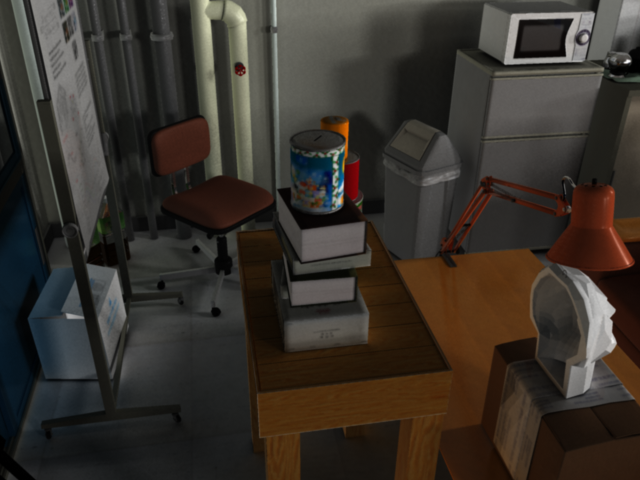
\includegraphics[width=0.40\textwidth]{./images/tsukuba_fluorescent_L_00313.png}
	} 
	\subfloat[Right image]{
		\label{fig:tsukuba_fluorescent_R_00313}
		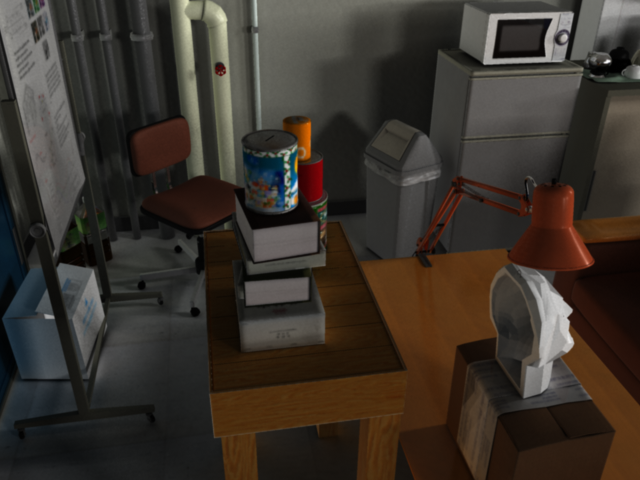
\includegraphics[width=0.40\textwidth]{./images/tsukuba_fluorescent_R_00313.png}
	} 
	\caption{Example image pair of New Tsukuba Stereo Dataset with scattered facets \cite{nakamuraOcclusionDetectableStereoocclusion1996}}
	\label{fig:tsukuba_fluorescent_00313}
\end{figure}
\begin{figure}[htbp]\centering
	\subfloat[Left Image]{
		\label{fig:tsukuba_fluorescent_L_00566}
		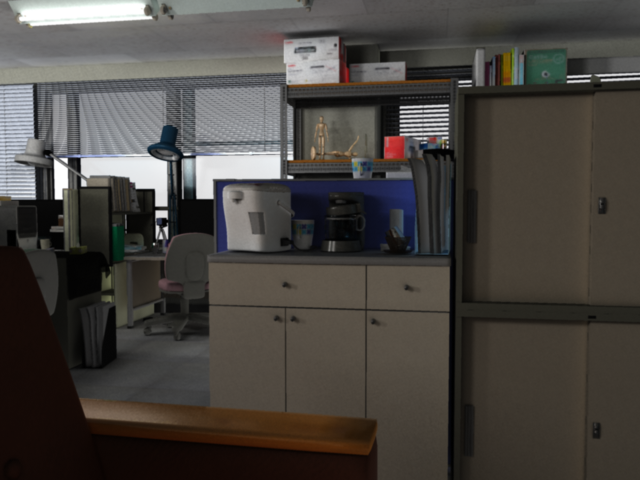
\includegraphics[width=0.40\textwidth]{./images/tsukuba_fluorescent_L_00566.png}
	} 
	\subfloat[Right Image]{
		\label{fig:tsukuba_fluorescent_R_00566}
		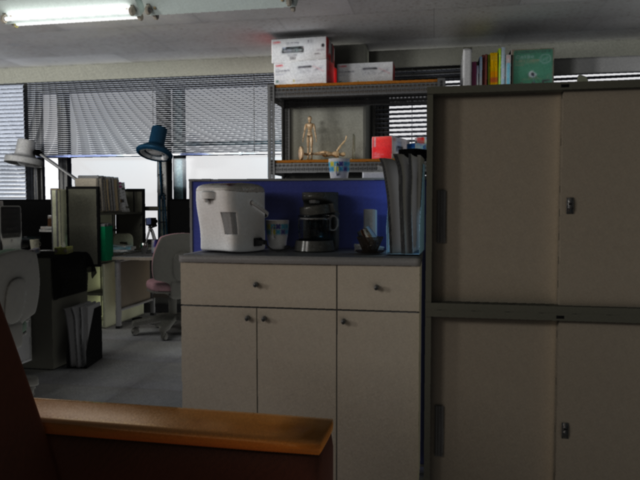
\includegraphics[width=0.40\textwidth]{./images/tsukuba_fluorescent_R_00566.png}
	} 
	\caption{Example image pair of New Tsukuba Stereo Dataset with no feature plane \cite{nakamuraOcclusionDetectableStereoocclusion1996}}
	\label{fig:tsukuba_fluorescent_00566}
\end{figure}

AdelaideRMF is a data set for robust geometric model fitting (homography estimation and fundamental matrix estimation). It collects a set of image pairs and the key-point correspondences which were obtained by SIFT matching are manually labeled\cite{wongDynamicHierarchicalMultistructure2011}. Unlike New Tsukuba Stereo Dataset, most of the scenes in it are different buildings, so there are a lot of large flat planes in images \cref{fig:ladysmomo}, such as the wall of red building.
\begin{figure}[htbp]\centering
	\subfloat[Left image]{
		\label{fig:ladysmom1}
		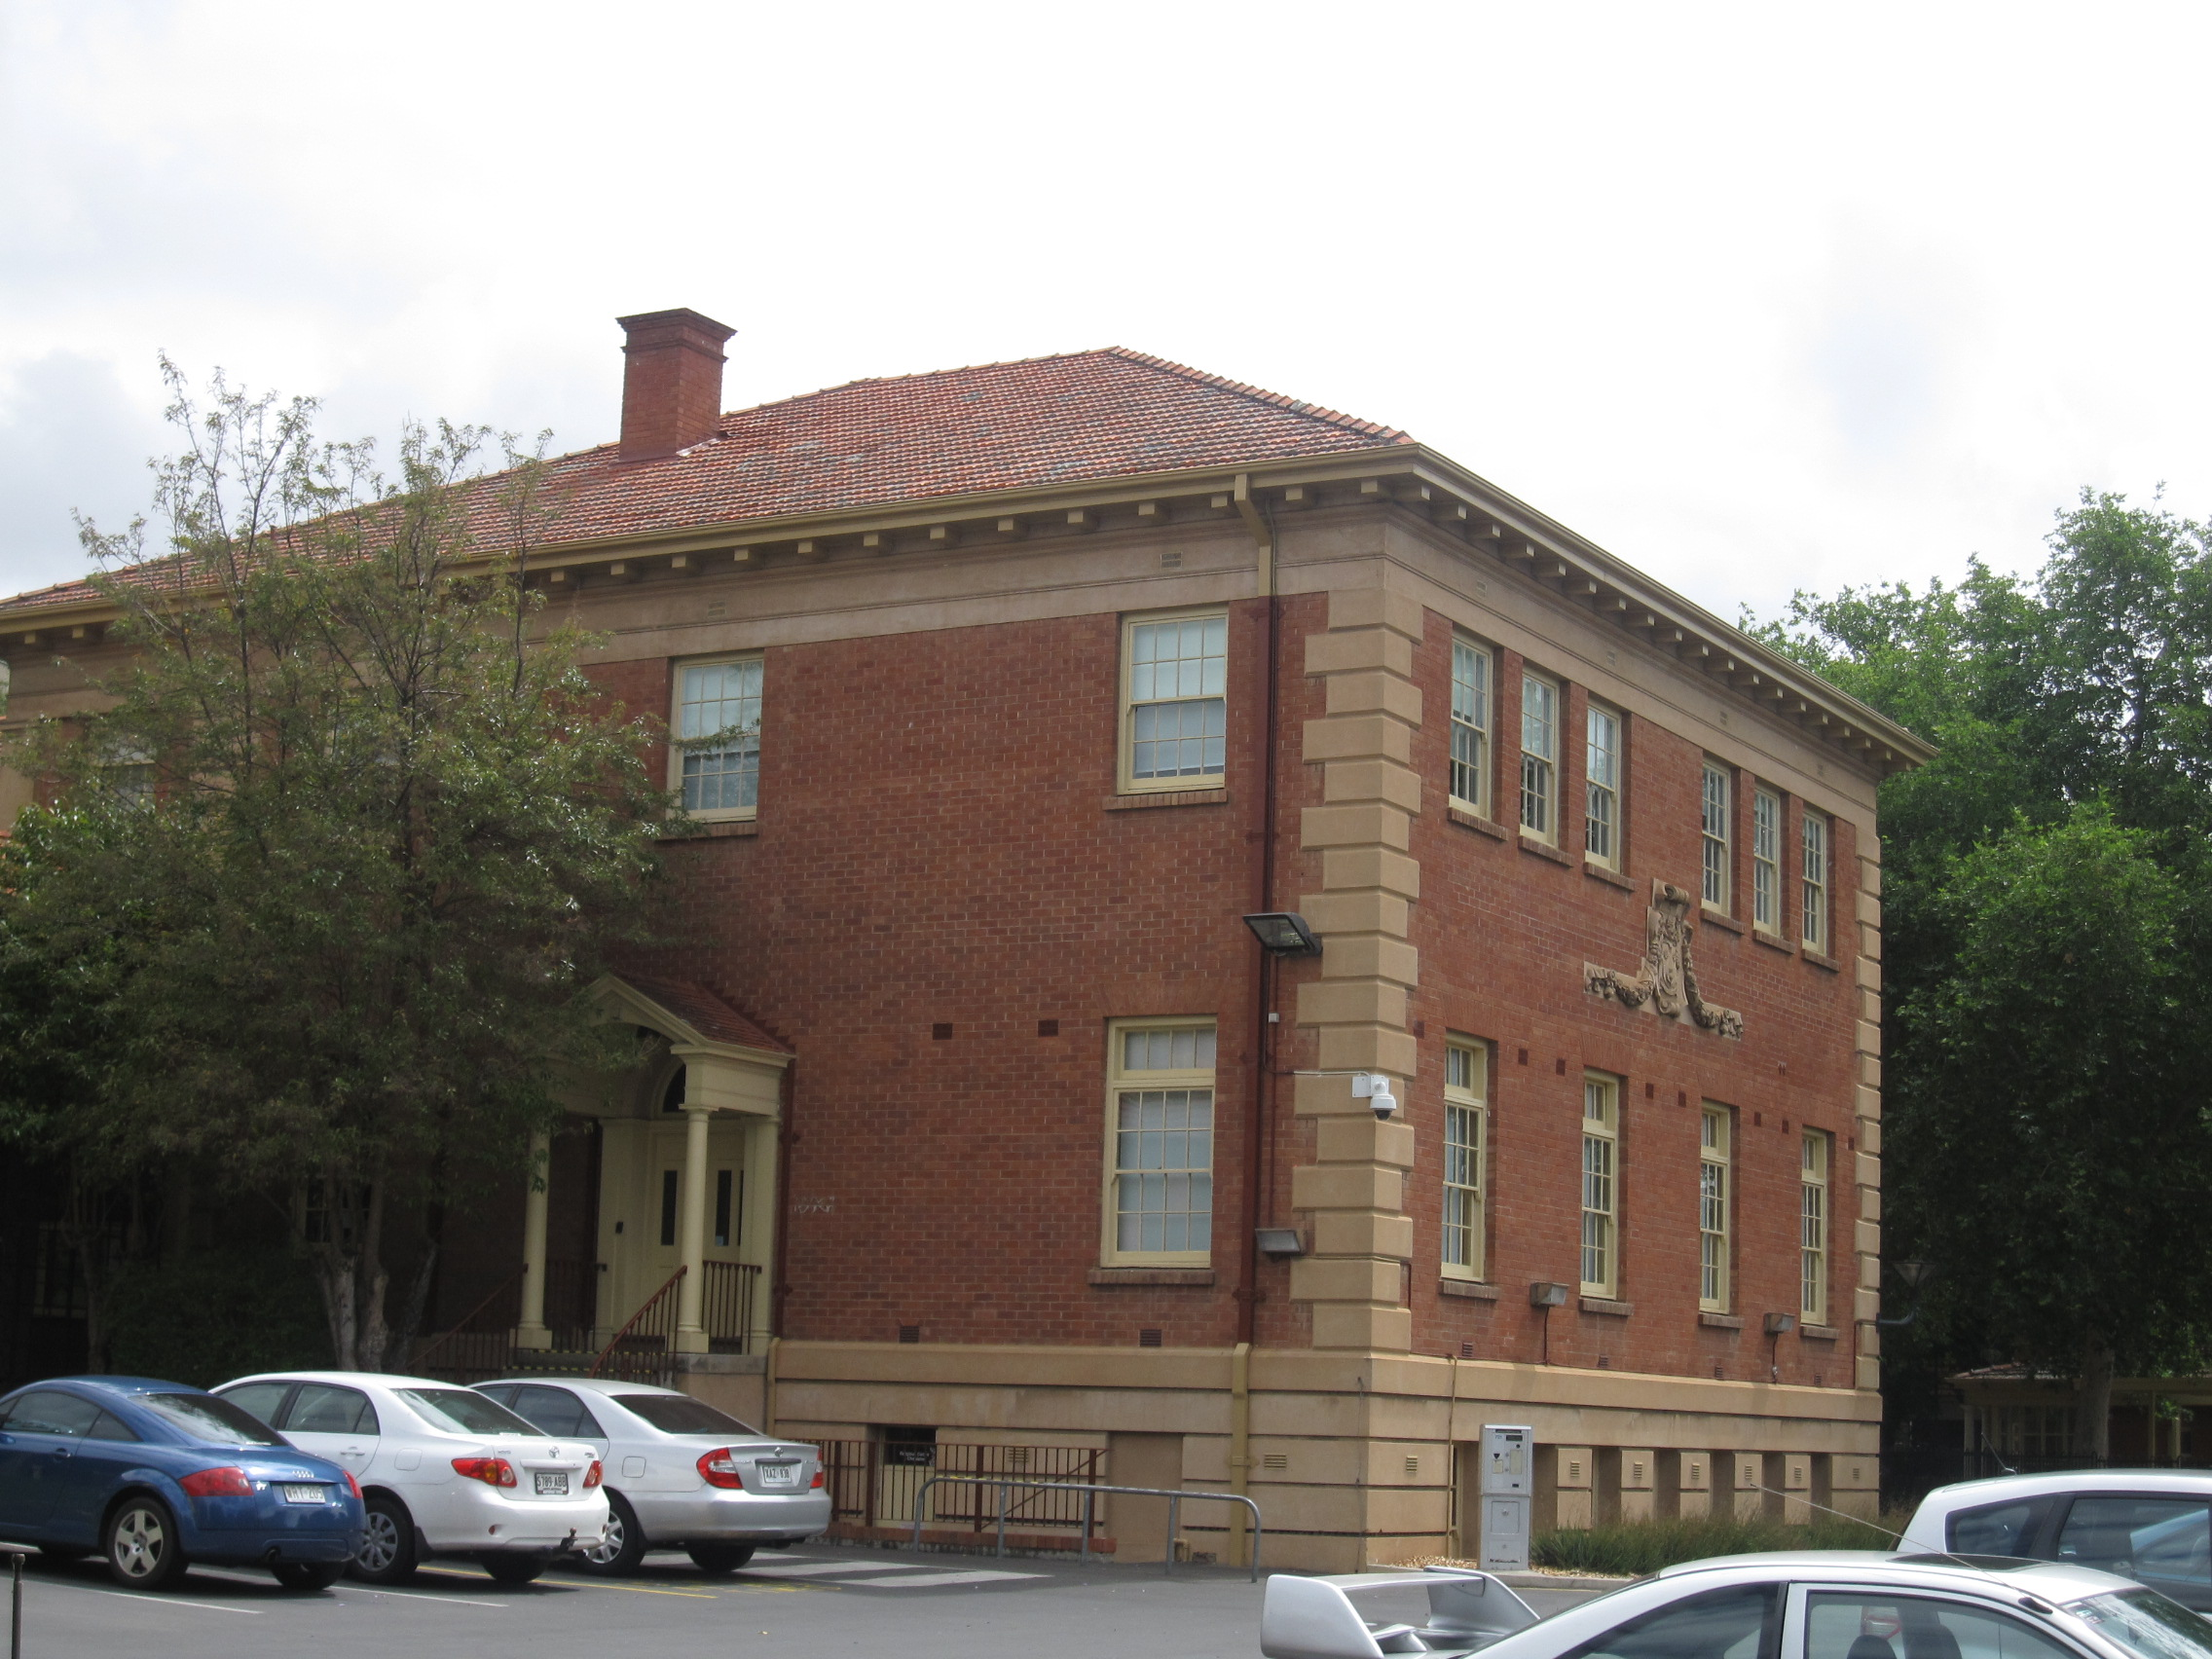
\includegraphics[width=0.50\textwidth]{./images/ladysmom1}
	} \hspace{-2mm}
	\subfloat[Right image]{
		\label{fig:ladysmom2}
		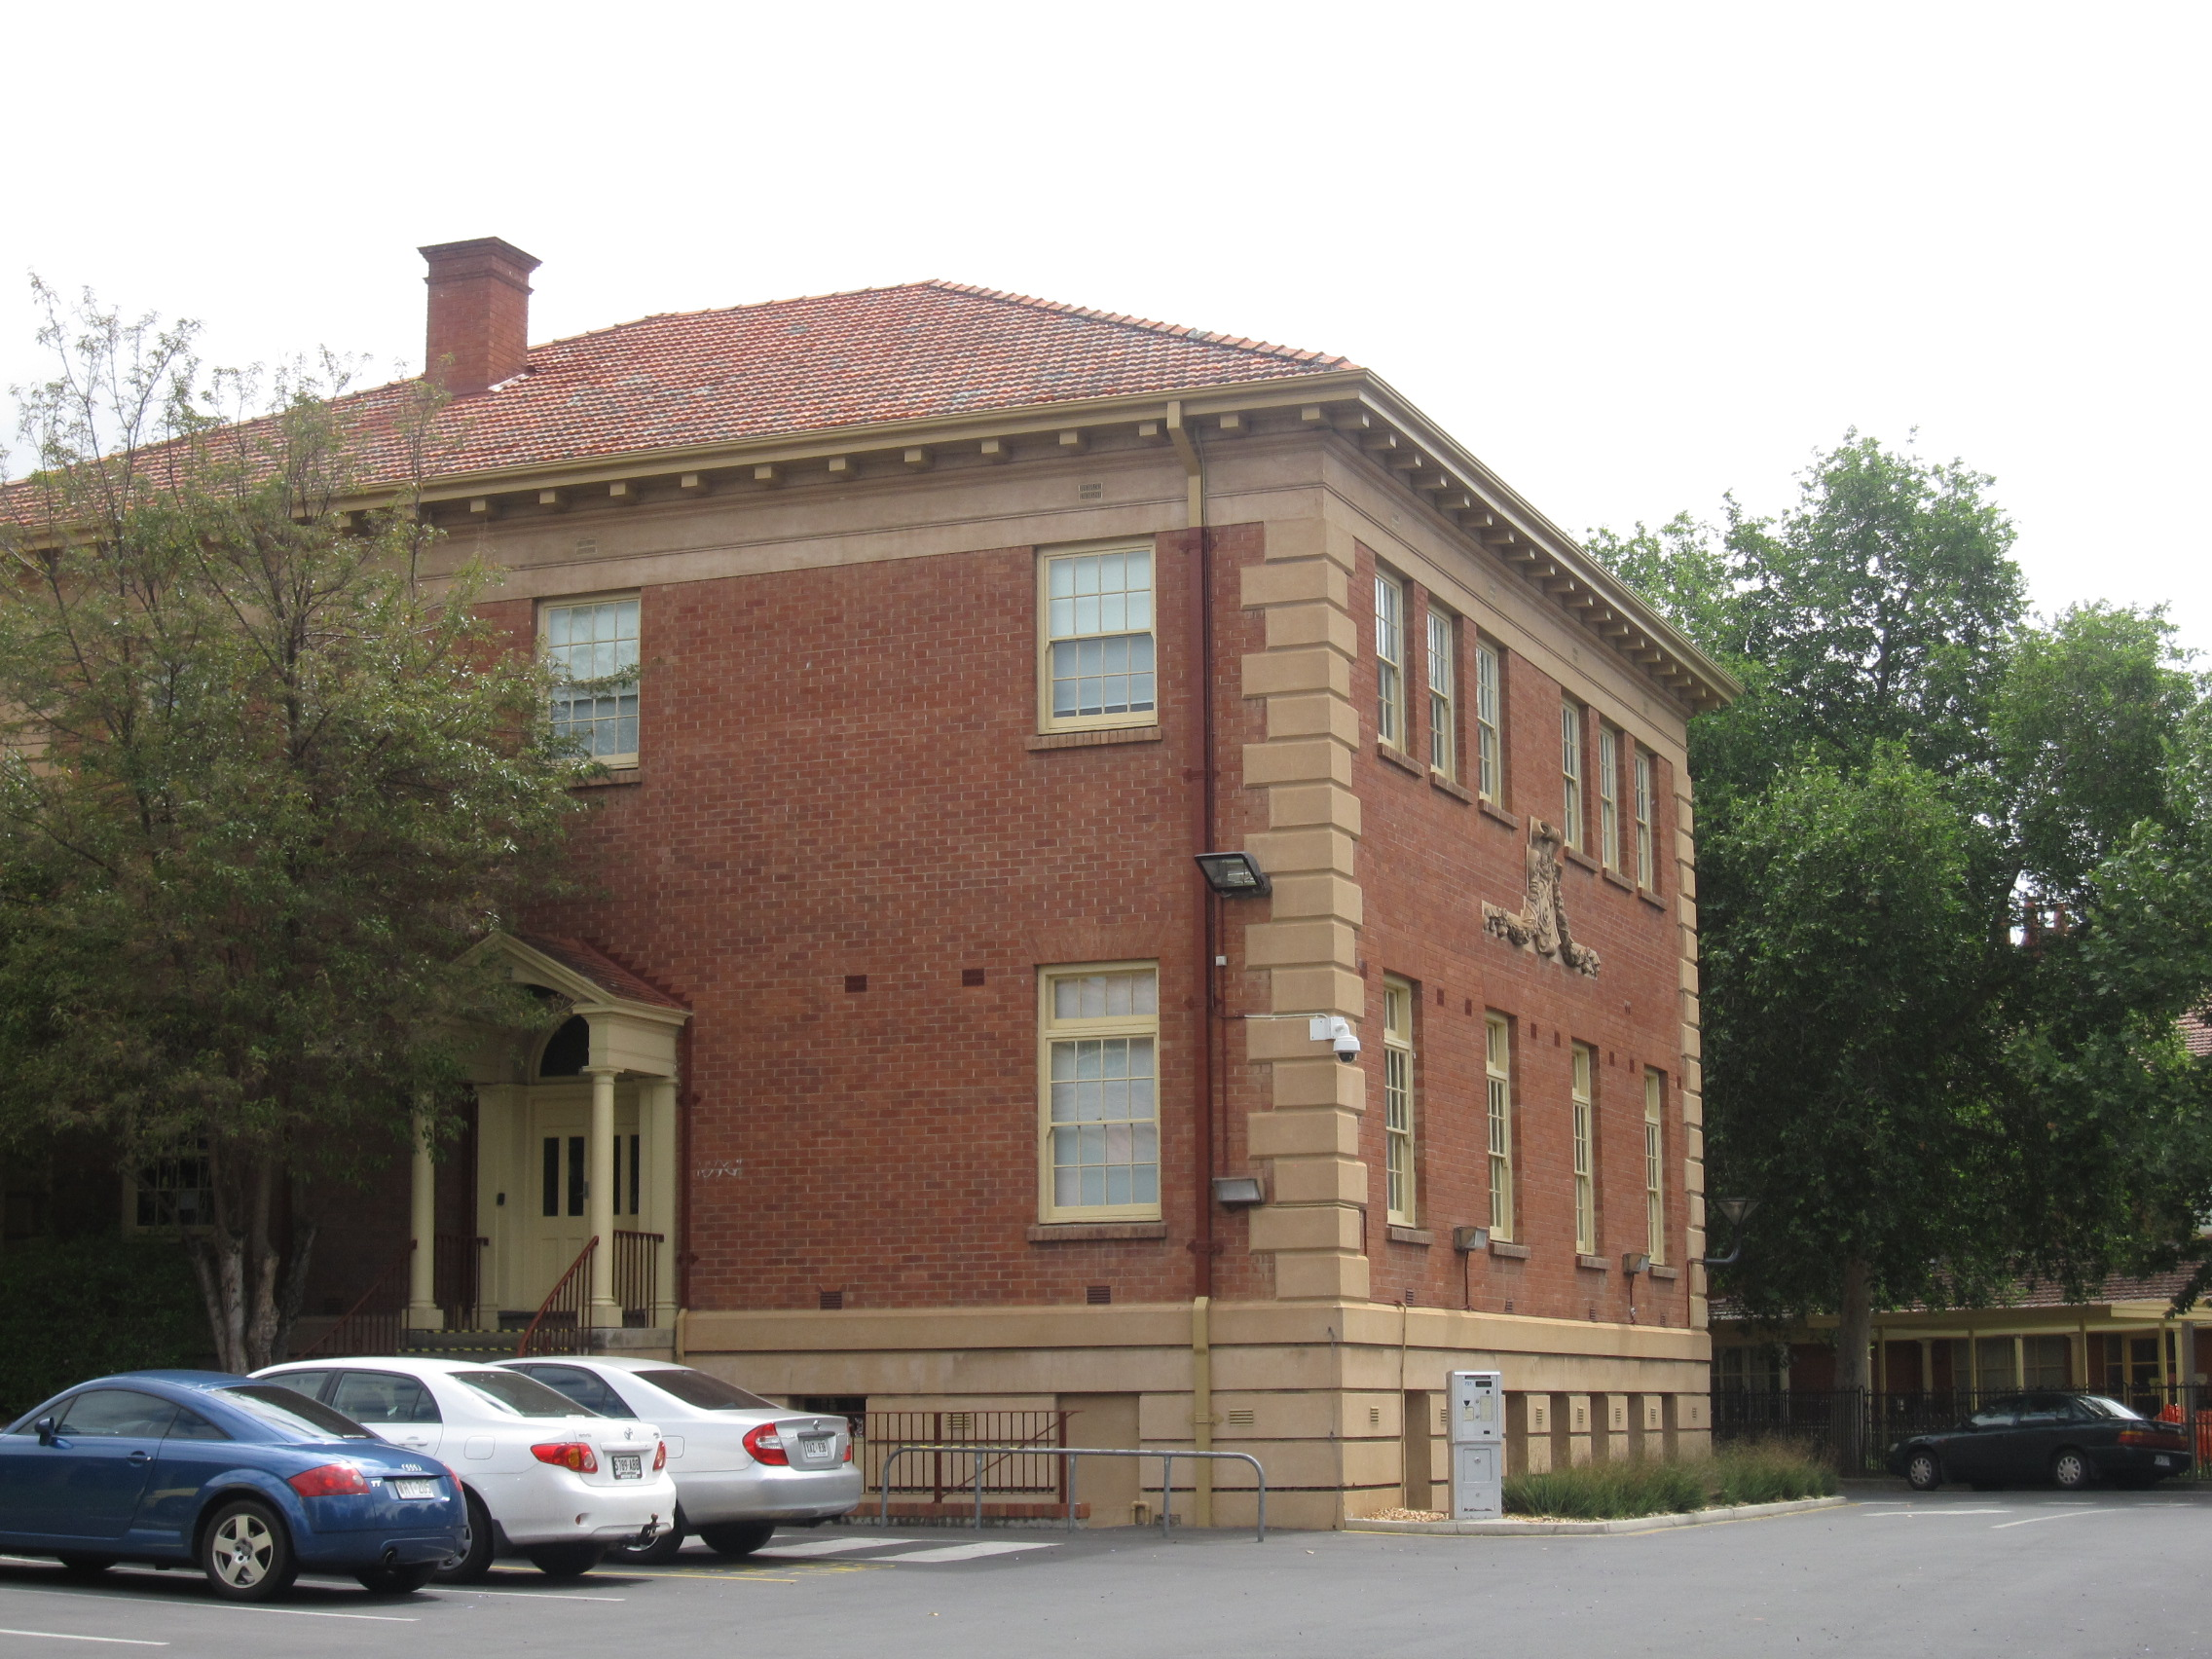
\includegraphics[width=0.50\textwidth]{./images/ladysmom2}
	} 
	\caption{Example image pair of AdelaideRMF Dataset \cite{wongDynamicHierarchicalMultistructure2011}}
	\label{fig:ladysmomo}
\end{figure}

The purpose of evaluation is to evaluate the result of my algorithm, then ground truth is needed for reference. But in AdelaideRMF, there are only matching features that were obtained by SIFT matching. And they can be used to to estimate the homography matrix. But this result is still an approximate value, not a ground truth. So it's meaningless to compare with this result. In other words, this data set can only be used to show the results of our algorithm, but not to verify the accuracy of our algorithm.
\begin{figure}[htbp]\centering
	\subfloat[Barn 1]{
		\label{fig:barn1}
		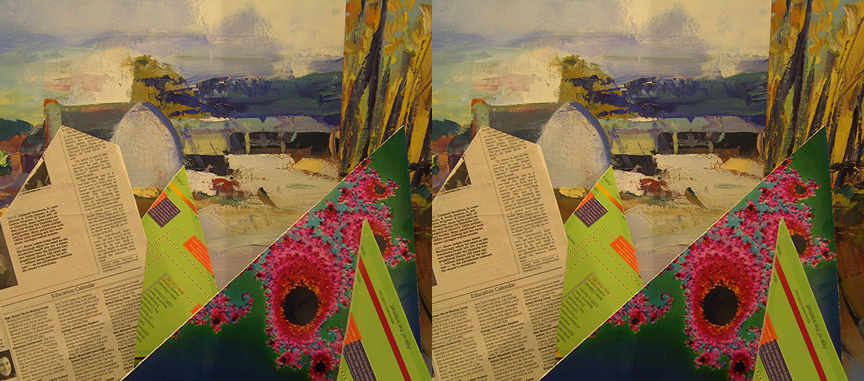
\includegraphics[width=0.60\textwidth]{./images/Middlebury_Stereo_Datasets/barn1.png}
	} \\
	\subfloat[Barn 2]{
		\label{fig:barn2}
		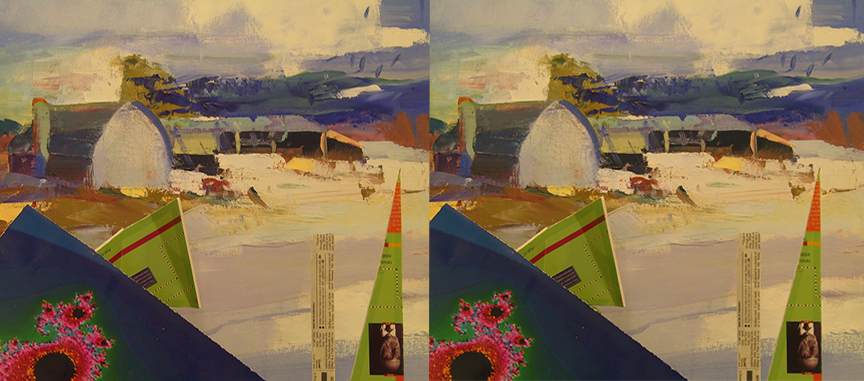
\includegraphics[width=0.60\textwidth]{./images/Middlebury_Stereo_Datasets/barn2.png}
	} \\
	\subfloat[Bull]{
		\label{fig:bull}
		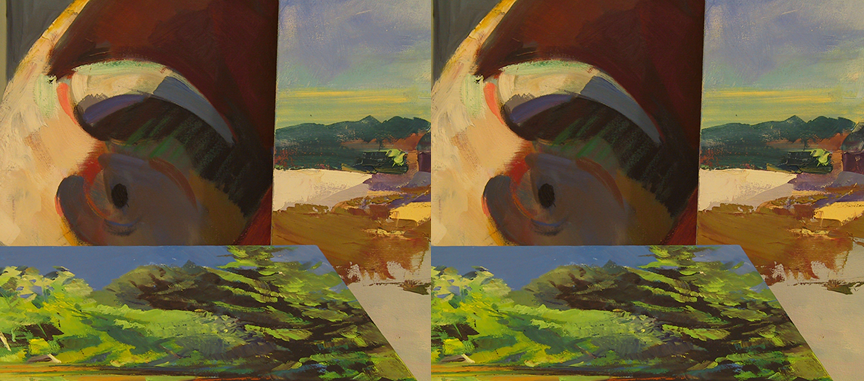
\includegraphics[width=0.60\textwidth]{./images/Middlebury_Stereo_Datasets/bull.png}
	}\\		
	\caption{Middlebury Stereo Vision Datasets 2001 Version(1) \cite{scharsteinTaxonomyEvaluationDense2001}}
	\label{fig: Middlebury Stereo Vision Datasets 2001 Version(1)}
\end{figure}

\begin{figure}
	
	\centering
	\subfloat[Poster]{
		\label{fig:poster}
		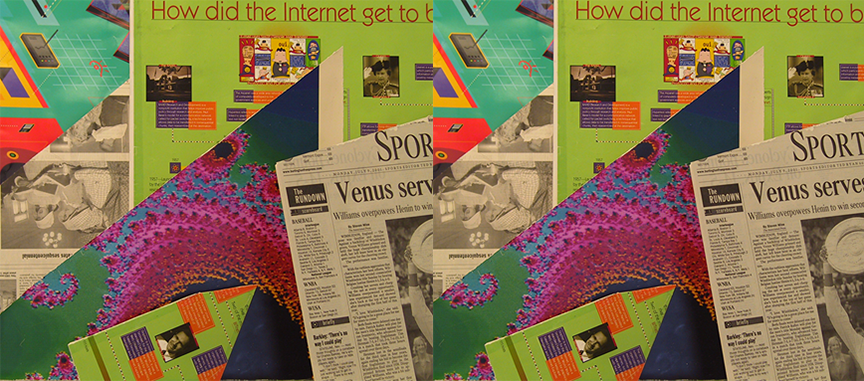
\includegraphics[width=0.60\textwidth]{./images/Middlebury_Stereo_Datasets/poster.png}
	} \\
	\subfloat[Swatooth]{
		\label{fig:swatooth}
		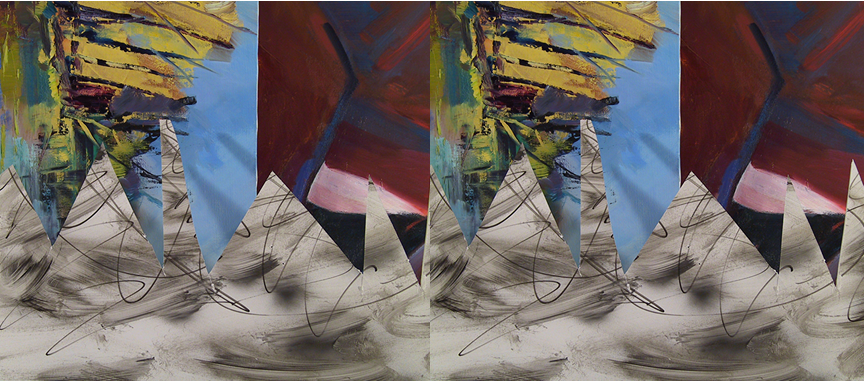
\includegraphics[width=0.60\textwidth]{./images/Middlebury_Stereo_Datasets/swatooth.png}
	} \\
	\subfloat[Venus]{
		\label{fig:venus}
		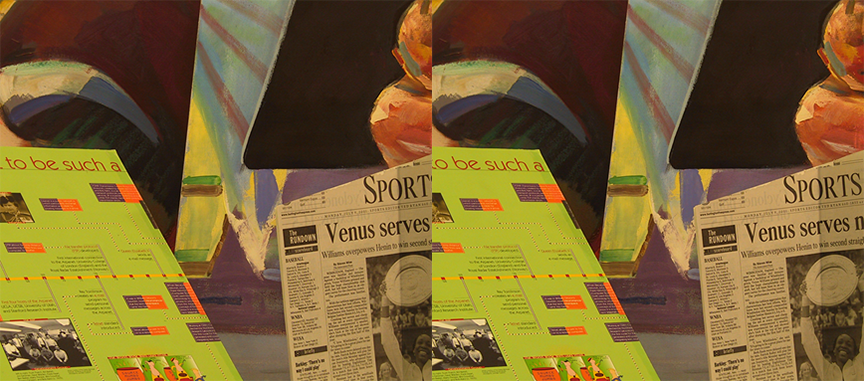
\includegraphics[width=0.60\textwidth]{./images/Middlebury_Stereo_Datasets/venus.png}
	} 
	\caption{Middlebury Stereo Vision Datasets 2001 Version(2) \cite{scharsteinTaxonomyEvaluationDense2001}}
	\label{Middlebury Stereo Vision Datasets 2001 Version(2)}
\end{figure}

In the end, I introduce Middlebury Stereo Vision Datasets. I mainly used the 2001 Stereo datasets in it with ground truth. There are 6 datasets of piecewise planar scenes \cref{fig: Middlebury Stereo Vision Datasets 2001 Version(1)} and \cref{Middlebury Stereo Vision Datasets 2001 Version(2)}. Because the image pairs in this dataset is all perfect rectified, they can only be use to evaluate the rectified case. 

Besides these stereo image datasets, there are also some available aerial image datasets. But the most datasets don't contain stereo images. Only a small part of them have stereo images, such as ASL Datasets  \url{http://projects.asl.ethz.ch/datasets/} and CMLA Subpixel Stereo Dataset  \url{http://www.ipol.im/pub/pre/187/}. But they either don't have flat plane structure, or they don't have a ground truth. So I don't consider them further.

Because the public datasets, that I could find, are only partly suited for the evaluation of the proposed algorithm. I decided to build my own dataset to verify the algorithm.
\section{Self-Built Datasets} \label{sec:Self-Built Datasets}
In order to construct our own dataset, I first need a virtual environment. I choose Blender as the software for the build environment. Blender is used to manage the 3D scene and do the rendering. There can be some exact objects built by Blender in the virtual environment. In our case, we only need the plane patches in the images. So I just put some planes, which are shading with some pictures, in the scene and render the realistic images. The whole dataset is available online at: \url{https://github.com/Zauberr/Multi-H-Dataset}

The interface of the software is shown in \cref{fig:Interface of Blender}
\begin{figure}[htbp]
	\centering
	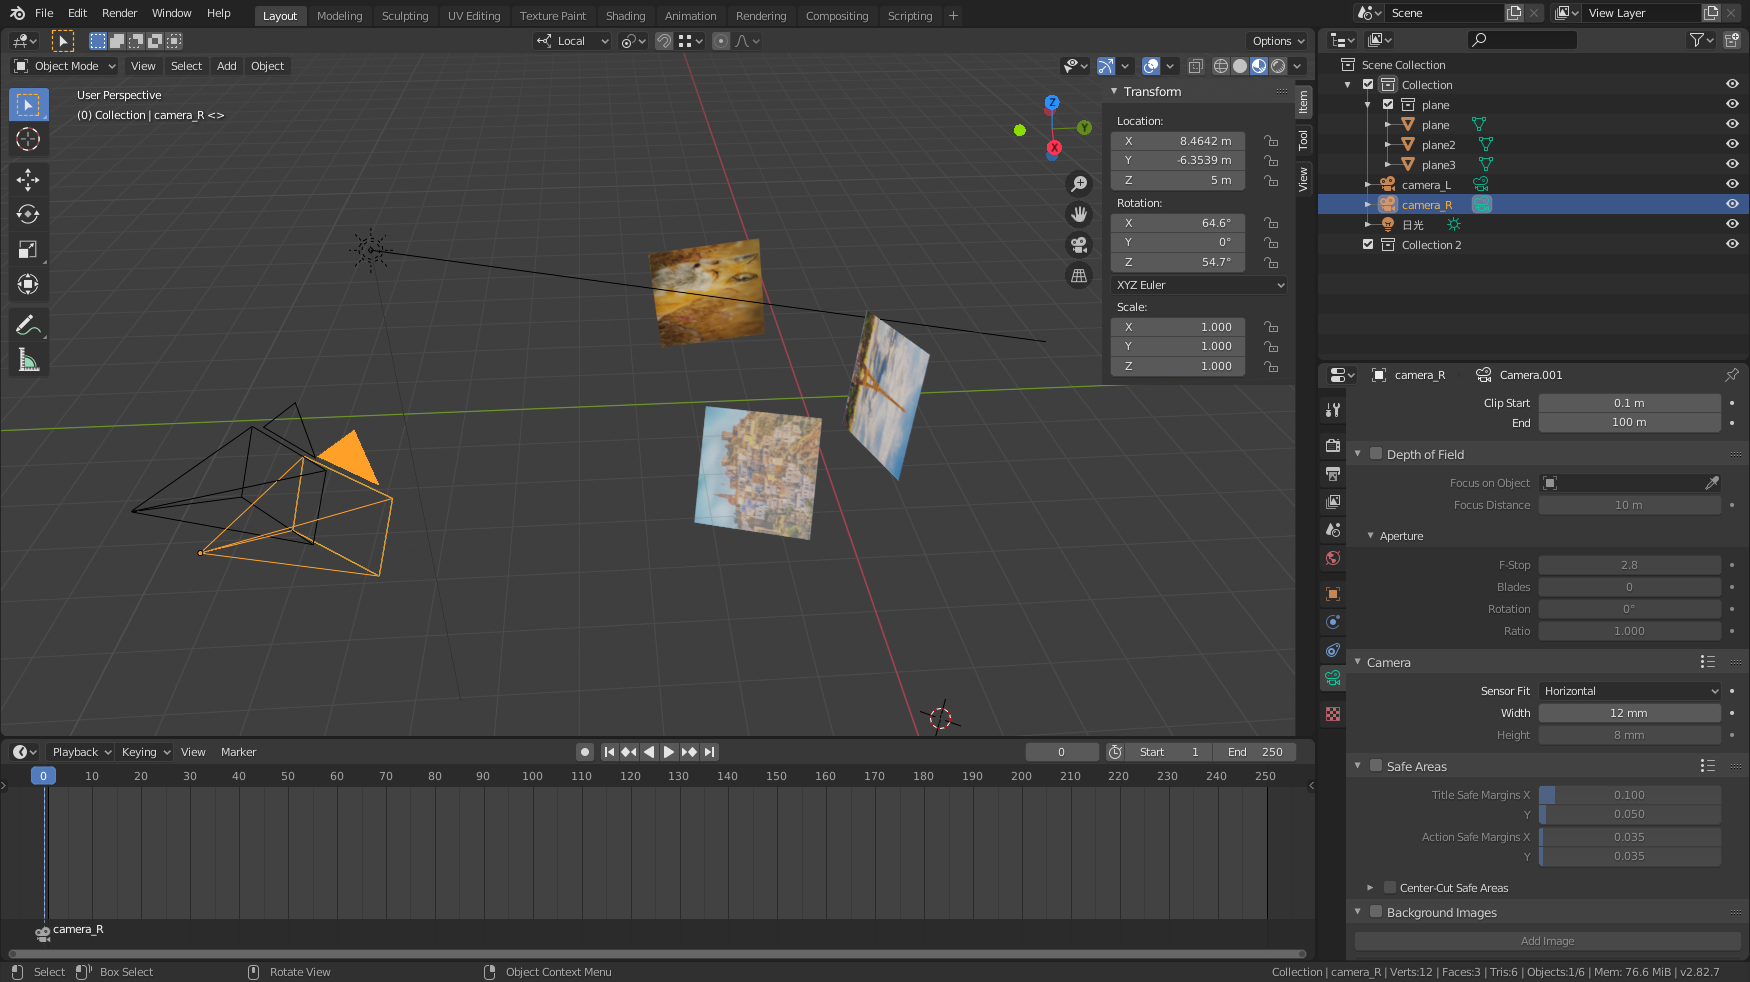
\includegraphics[width=0.80\textwidth]{images/Blender/software_interface.png}
	\caption{Interface of Blender}
	\label{fig:Interface of Blender}
\end{figure}

We can see from it that the central main interface is a constructed virtual scene, in which the world coordinate system is preset, red is the x-axis, green is the y-axis and blue is the z-axis. Each object (rigid body) has its own position coordinates and rotation parameters relative to the world coordinate system. In the toolbar at bottom right corner of the screen, we can set the specific parameters of each object in detail. For example, for the camera we use, we can choose different camera models and different focal lengths, etc.

After understanding the main software situation, we focus on the processing pipeline of dataset. We will use the scene in \cref{fig:Interface of Blender} as an example to explain the entire process in detail. First of all, because the algorithm applies to plane structures, we first put three plane structures in the scene and draw different patterns on the surface of each picture. We  call the plane showing the fox the "fox plane", showing Eiffel Tower "eiffel plane" and the last one "greece plane". (In the whole datasets, the used images are from \url{https://pixabay.com}.) The transformations of these three planes are shown in the \cref{fig:Transformation of example planes}.
\begin{figure}[tbp]
	\centering
	\subfloat[Fox]{
		\label{fig:fox}
		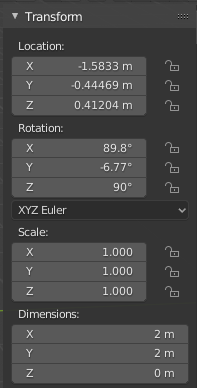
\includegraphics[width=0.20\textwidth]{./images/Blender/brickwall}
	} \quad
	\subfloat[Eiffel Tower]{
		\label{fig:Eiffel Tower}
		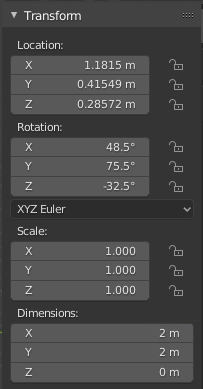
\includegraphics[width=0.20\textwidth]{./images/Blender/voronoi_plane}
	} \quad
	\subfloat[Greece]{
		\label{fig:Greece}
		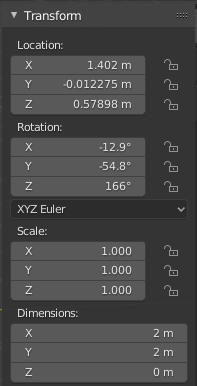
\includegraphics[width=0.20\textwidth]{./images/Blender/markov_plane}
	}
	\caption{Transformation of example planes}
	\label{fig:Transformation of example planes}
\end{figure}

After successfully building the scene with the images, we need to extract the image data (render the image) from the virtual scene. In this step we use the camera components in the software. We placed a pair of stereo camera equipment consisting of two cameras with identical internal parameters (shown in \cref{fig:Inter-parameter of Stereo Cameras}) in front of three planes. 
\begin{figure}[htbp]
	\centering
	\subfloat[]{
		\label{fig:inter_parameter1}
		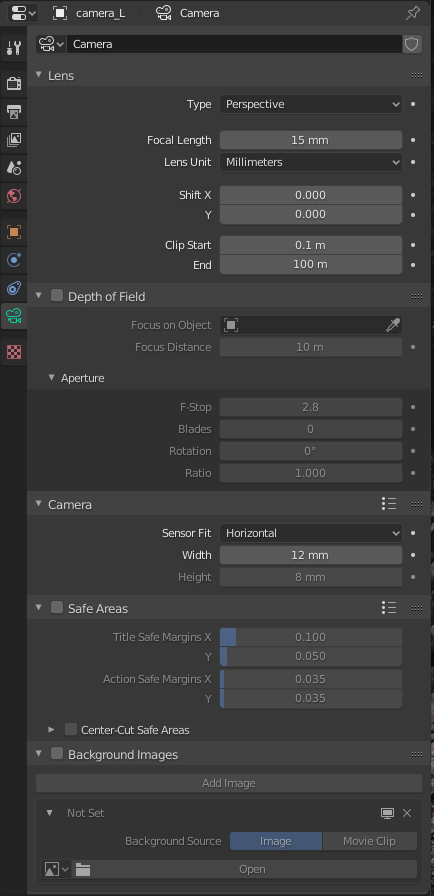
\includegraphics[width=0.40\textwidth]{./images/Blender/camera_inter_parameter}
	} \quad
	\subfloat[]{
		\label{fig:inter_parameter2}
		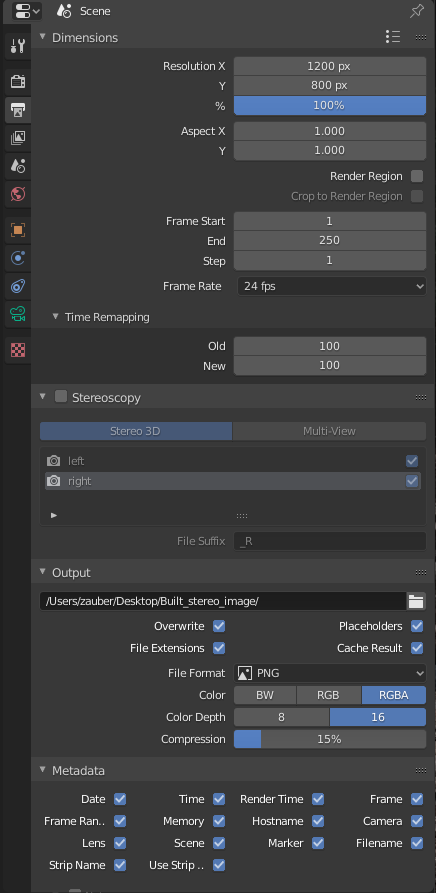
\includegraphics[width=0.40\textwidth]{./images/Blender/camera_inter_parameter2}
	} 
	\caption{Internal parameter of stereo cameras}
	\label{fig:Inter-parameter of Stereo Cameras}
\end{figure}

The calculation of imaging process also requires external parameters of the camera, such as rotation and translation. These parameters can also be obtained in the software. The parameters in the example are shown in \cref{fig:External-parameter of Stereo Cameras}
\begin{figure}[htbp]
	\centering
	\subfloat[Left Camera]{
		\label{fig:external_parameter1}
		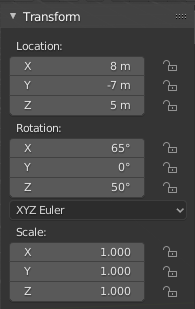
\includegraphics[width=0.30\textwidth]{./images/Blender/camera_external_parameter}
	} \quad
	\subfloat[Right Camera]{
		\label{fig:external_parameter2}
		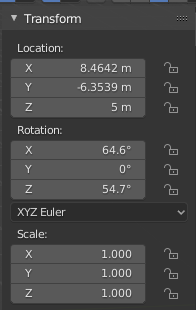
\includegraphics[width=0.30\textwidth]{./images/Blender/camera_external_parameter2}
	} 
	\caption{External-parameter of stereo cameras}
	\label{fig:External-parameter of Stereo Cameras}
\end{figure}

After providing the light source in the scene, we have completed the construction of a simple virtual environment. After that, the scene should be rendered and collect the raw image data, which can be automatic done by the software. Next, we need to get the specific imaging formula corresponding to our image and the homography matrix of the plane in it, which is regarded as ground truth.

The specific imaging process and formula are exactly the same as described in \cref{sec:main idea}. Finally, we use the \cref{eq:Multiplehomographymatri} to solve homography matrix for each plane. And here I add how to get the parameter matrices needed in \cref{eq:Multiplehomographymatri} based on the actual virtual environment parameters.

For convenience, \cref{eq:Multiplehomographymatri} is repeated here:
\begin{align}
	H=K_{2}R_{2}^T R_{1}K_{1}^{-1}+K_{2}R_{2}^T(\rdc_{1}-\rdc_{2})\cdot \frac{\vec{n}_n^{T}}{d_n}R_{1}K_{1}^{-1}\nonumber
\end{align}
where 
\begin{itemize}
	\item $\rdc_{1},\rdc_{2}$ : location of the camera center in the world coordinate system
	\item $R_{1},R_{2}$: rotation matrix of world coordinate system relative to the camera
	\item $K_{1},K_{2}$: calibration matrix of camera
	\item $\vec{n}_n$: unit outward normal vector of plane
	\item $d_n$: distance from the plane to camera center $C_1$
\end{itemize}

I use the virtual scene shown previously as an example to solve each parameter separately in the equation. In the process of solving each parameter, the meaning of parameters in the formula is the same as the  meaning in each source picture. And the left camera is camera 1.
\begin{itemize}
	\item {\Large $\rdc_{1},\rdc_{2}$}: \\
	From \cref{fig:External-parameter of Stereo Cameras}, we can get the transform information for stereo camera pairs. we can use the location information shown to describe $\rdc_{1},\rdc_{2}$:
	\begin{align}
		\rdc = \begin{bmatrix}
		X\\
		Y\\
		Z
		\end{bmatrix}= \begin{bmatrix}8 \\-7\\5 \end{bmatrix}
	\end{align}
	\item {\Large $R_{1},R_{2}$}: \\
	From \cref{fig:External-parameter of Stereo Cameras}, we can get the transform information for stereo camera pairs. we can use the Rotation information shown to describe $R_{1},R_{2}$ \cite{bernerTechnicalConceptsOrientation2008}, and in blender, it uses extrinsic parameters, in other words, space-fixed rotation.
	\begin{align}
		R &= R_z(Z) R_y(Y) R_x(X) \nonumber \\
			& = R_z(50^{\circ}) R_y(0^{\circ}) R_x(65^{\circ}) \nonumber \\
			& = \begin{bmatrix}
			\cos Z \cos Y & \cos Z \sin Y \sin X - \sin Z \cos X& \cos Z \sin Y \cos X + \sin Z \sin X\\
			\sin Z \cos Y & \sin Z \sin Y \sin X + \cos Z \cos X & \sin Z \sin Y \cos X -\cos Z \sin X \\
			-\sin Y& \cos Y \sin X& \cos Y \cos X
		\end{bmatrix}
	\end{align}

	\item {\Large $K_{1},K_{2}$}: \\
	From \cref{fig:Inter-parameter of Stereo Cameras}, we can get the focal length of camera $f$, sensor width $x$, sensor height $y$ and resolution $X$ and $Y$. The output pixel in the image is set as squared pixel. The scaling factors $k_{x}, k_{y}$ are
	\begin{align}
		k_{x} = k_{y} = \frac{\sqrt{X^2 + Y^2}}{\sqrt{x^2 + y^2}} = \frac{\sqrt{1200^2 + 800^2}}{\sqrt{12^2 + 8^2}} = 100 px/mm 
	\end{align}
	then $K_{1},K_{2}$:
	\begin{align}
	K = K_{1}=K_{2} = \begin{bmatrix}
	f k_{x} & 0 & \frac{X-1} {2} & 0 \\
	0 & -f k_{y} &  \frac{Y-1} {2} & 0 \\
	0 & 0 & -1 & 0
	\end{bmatrix} 
	\end{align}
	where the minus for $f k_{y}$ and $1$ comes from converting coordinate between right-up-backwards coordinate system of Blender and right-down-forward coordinate system of OpenCV.
	
	\item {\Large $\vec{n}_n$}: \\
	From \cref{fig:Transformation of example planes}, we can get location and rotation of each plane. And the unit outward normal vector of each plane before transformation is set by software $\vec{n}_{init} = (0, 0, 1)^T$. So $\vec{n}_n$:
	\begin{align}
		\vec{n} &= R_{plane} \cdot \vec{n}_{init} \nonumber \\
						&= \begin{bmatrix}
							\cos Z \cos Y & \cos Z \sin Y \sin X - \sin Z \cos X& \cos Z \sin Y \cos X + \sin Z \sin X\\
							\sin Z \cos Y & \sin Z \sin Y \sin X + \cos Z \cos X & \sin Z \sin Y \cos X -\cos Z \sin X \\
							-\sin Y& \cos Y \sin X& \cos Y \cos X
						\end{bmatrix} \begin{bmatrix}
						0\\0\\1
						\end{bmatrix}
	\end{align}
	\item {\Large $d_n$}: \\
	Here we regard the right camera as the camera 1. From \cref{fig:external_parameter2}, we know the location of the camera 1 $\rdc_1$ and from \cref{fig:Transformation of example planes}, we can get a point $\vec{t} = (1, -1, 1)^T$ on the plane, which is the same as location of plane. So $d_n$:
	\begin{align}
	d_n = \vec{n}_n^T \rdc_1 - \vec{n}_n^T \vec{t}
	\end{align}
\end{itemize}

Combine all the equation above, we can finally calculate the ground truth: 
\begin{itemize}
	\item $H_{\infty}=K_{2}R_{2}R_{1}^{T}K_{1}^{-1}$
	\item $\vec{e}=K_{2}R_{2}(\rdc_{1}-\rdc_{2})$
	\item $\vec{q}_{n}^T=\frac{\vec{n}_n^{T}}{d_n}R_{1}^{-1}K_{1}^{-1}$
	\item $ H_{n} = H_{\infty} + \vec{e} \cdot \vec{q}_{n}^T$
\end{itemize}

\section{Testing}
After completing the collection and pre-processing of the public datasets and the construction of the test dataset, we could use these images to test my algorithm. In this section, some testing results of the algorithm is shown.
\subsection{Testing with Middlebury Stereo Vision Datasets}\label{subsec:Testing with Middlebury Stereo Vision Datasets}
First, we apply my algorithm on the dataset of Middlebury Stereo Vision Datasets 2001 Version. Just like mention before, the images in the dataset are all rectified. So we use it only to test the rectified case of the algorithm. The results of all image pairs are shown in \cref{fig:Template and transformed plane patches in Middlebury Stereo Vision Datasets} and the PSNR are shown in \cref{tab:PSNR of different patches in  Middlebury Stereo Vision Datasets}. The root mean squared displacement (RMSD) of all patches are shown in \cref{tab:Displacement of different patches for self-built images (1)}.

It can be seen from the results that when the algorithm is applied to the rectified stereo images very stable. That is to say, when $H_{\infty}$ and $\rde$ are known, the result is usually quite accurate. 

\begin{figure}[htbp]\centering
	\subfloat[]{
		\label{fig:Template and transformed plane patches in Middlebury Stereo Vision Datasets (1)}
		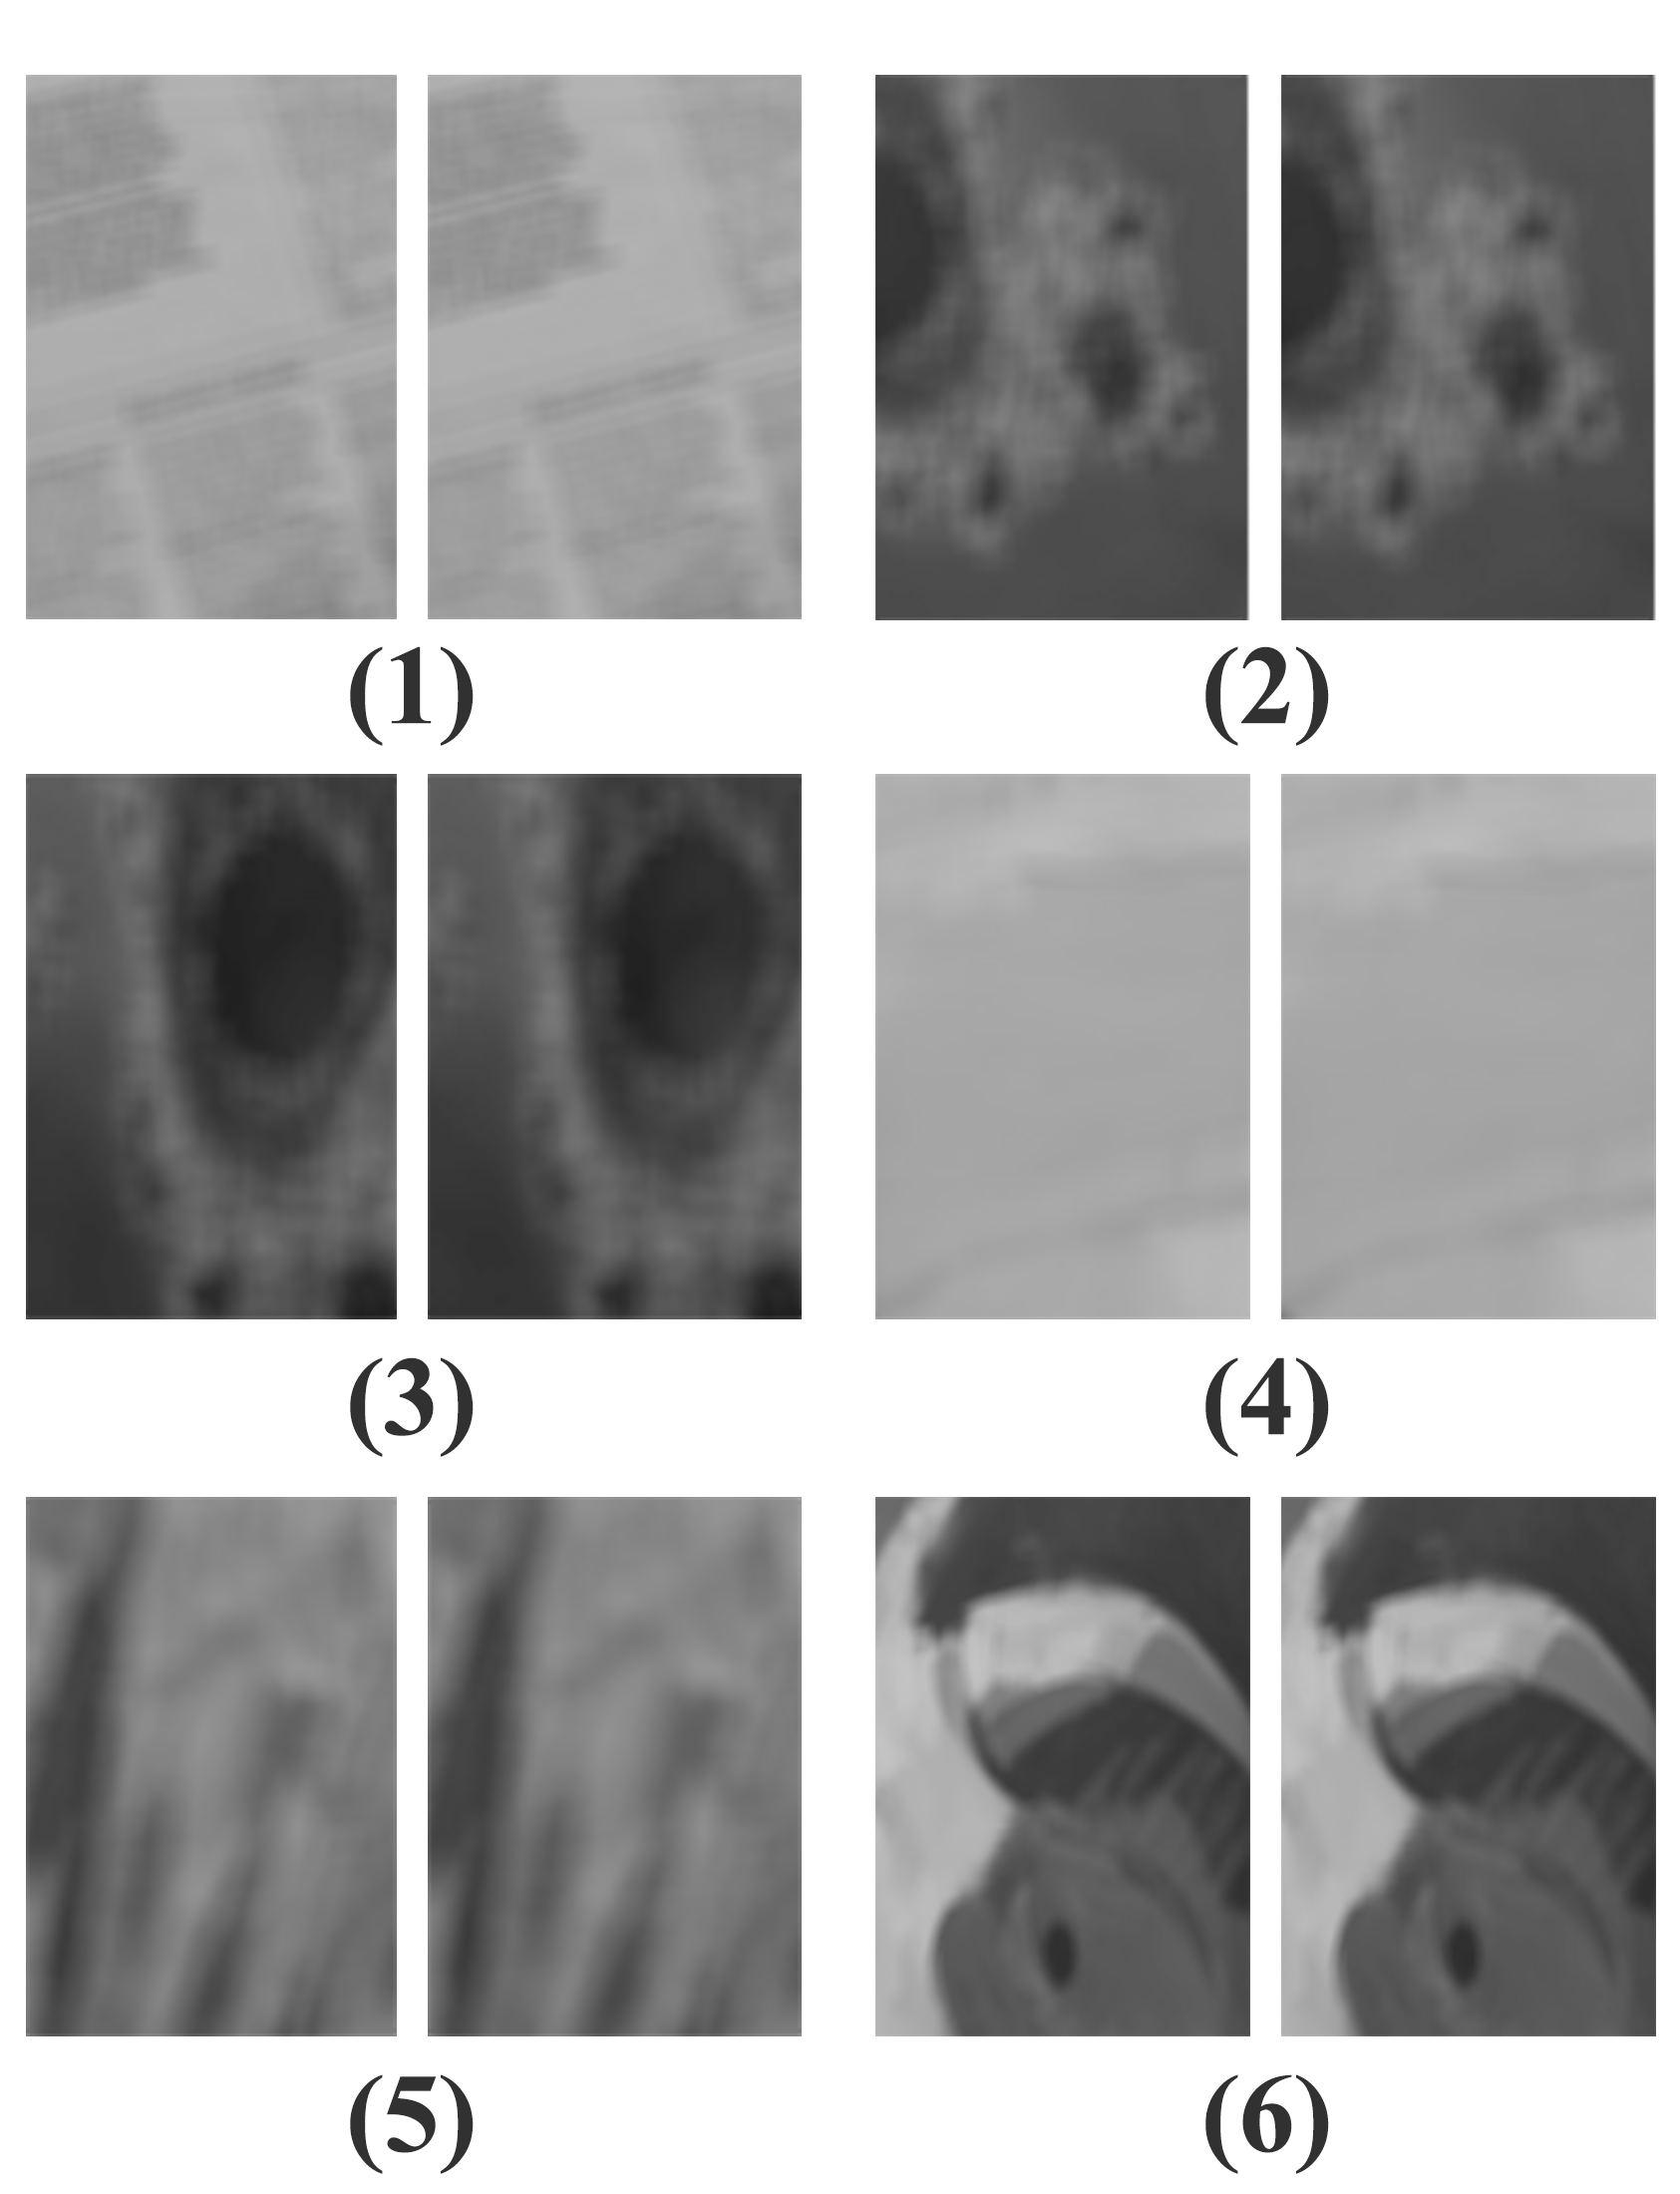
\includegraphics[width=0.40\textwidth]{images/Middlebury_Stereo_Datasets/shown1}
	} 
	\subfloat[]{
			\label{fig:Template and transformed plane patches in Middlebury Stereo Vision Datasets (2)}
		\includegraphics[width=0.40\textwidth]{images/Middlebury_Stereo_Datasets/shown2}
	} \\
		\subfloat[]{
		\label{fig:Template and transformed plane patches in Middlebury Stereo Vision Datasets (3)}
		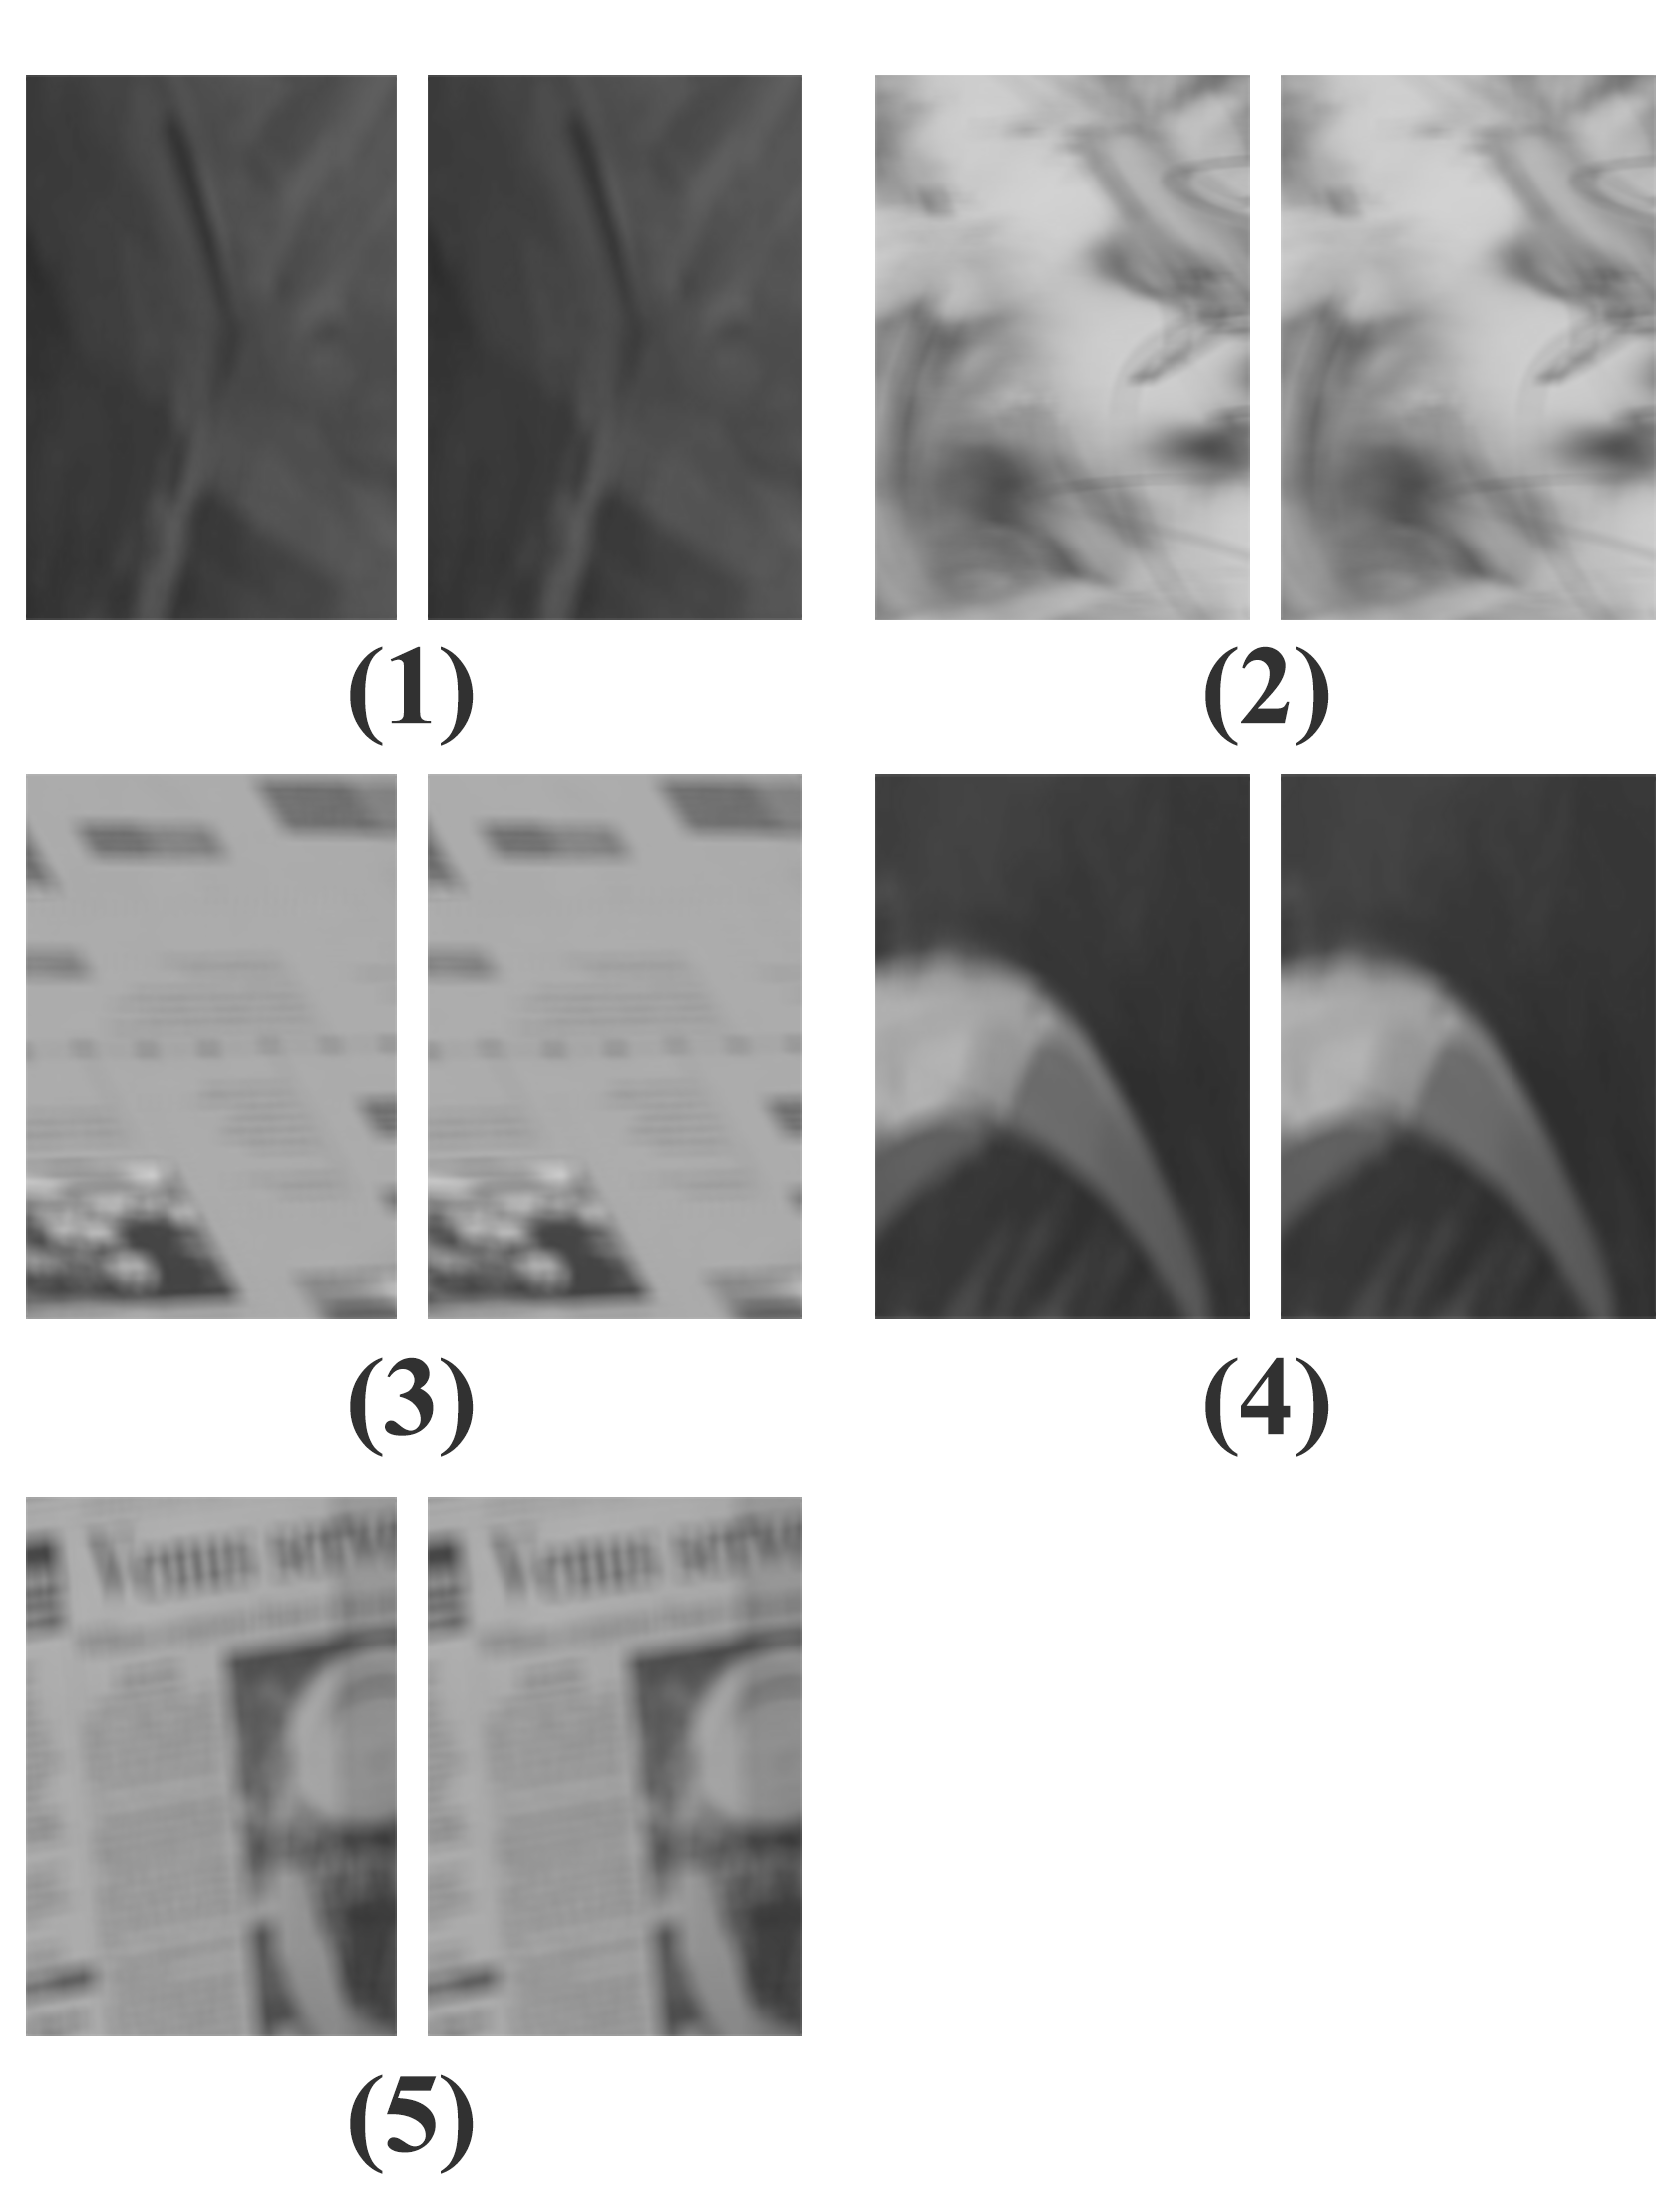
\includegraphics[width=0.40\textwidth]{images/Middlebury_Stereo_Datasets/shown3}
	} 
	\caption{Template and transformed plane patches in Middlebury Stereo Vision Datasets}
	\label{fig:Template and transformed plane patches in Middlebury Stereo Vision Datasets}
\end{figure}

\begin{table}[htbp]
	\centering
	\scriptsize  
	\begin{tabular}{ccccccc} 
		\hline 
		\multicolumn{1}{c}{\multirow{2}{1.2cm}{Shown Figure}} 
		&\multicolumn{5}{c}{Display Patch}  \\ 
		\cline{2-7} 
		&\multicolumn{1}{c}{(1)} & {(2)} & {(3)} & {(4)} & {(5)} & {(6)} \\ 
		\hline 
		\cref{fig:Template and transformed plane patches in Middlebury Stereo Vision Datasets (1)} &37.5768&40.4451&45.9941&42.4099&47.7764&38.3245 \\ 
		\cref{fig:Template and transformed plane patches in Middlebury Stereo Vision Datasets (2)}&46.9869&41.8912&32.6315&41.8892&36.9338&49.0576\\ 
		 \cref{fig:Template and transformed plane patches in Middlebury Stereo Vision Datasets (3)}&51.4393&44.9664&34.969591&47.4049&45.2209&\\ 
		\hline 
	\end{tabular} 
	\caption{PSNR (dB) of different patches in  Middlebury Stereo Vision Datasets}  
	\label{tab:PSNR of different patches in  Middlebury Stereo Vision Datasets} 
\end{table}

\begin{table}[htbp]
	\centering
	\scriptsize  
	\begin{tabular}{ccccccc} 
		\hline 
		\multicolumn{1}{c}{\multirow{2}{1.2cm}{Shown Figure}} 
		&\multicolumn{5}{c}{Display Patch}  \\ 
		\cline{2-7} 
		&\multicolumn{1}{c}{(1)} & {(2)} & {(3)} & {(4)} & {(5)} & {(6)} \\ 
		\hline 
		\cref{fig:Template and transformed plane patches in Middlebury Stereo Vision Datasets (1)} &2.252596&0.647761&0.184386&0.536102&0.954197&0.895281\\ 
		\cref{fig:Template and transformed plane patches in Middlebury Stereo Vision Datasets (2)}&0.203423&1.123935&1.523684&0.358562&1.111534&0.102031\\ 
		\cref{fig:Template and transformed plane patches in Middlebury Stereo Vision Datasets (3)}&0.507921&0.344584&1.353465&0.664646&0.188721&\\ 
		\hline 
	\end{tabular} 
	\caption{Displacement (pixel) of different patches in  Middlebury Stereo Vision Datasets}  
	\label{tab:Displacement of different patches in  Middlebury Stereo Vision Datasets} 
\end{table}

\subsection{Testing with Self-built Stereo Images}\label{subsec:Testing with Self-built Stereo Images}
When the algorithm is applied to the image pair without ground truth, the evaluation could only be done with the difference image and PSNR. Next, we will focus on application on the self-built testing images with ground truth. The evaluation can be done with the ground truth.

I start also with the rectified stereo images. The built images is shown in \cref{fig:Self-built Stereo Images}. And the ground truth of it was calculated in the way mentioned in \cref{sec:Self-Built Datasets}. Using algorithm on the images, the result is shown in \cref{fig:Result of Self-built Stereo Images} and the estimated parameters are in \cref{tab:Ground Truth and Estimated Parameter for self-built Stereo Images}. PSNR is in \cref{tab:PSNR of different patches for Self-built Stereo Images}. The root mean squared displacement (RMSD) and maximum displacement of all patches are shown in \cref{tab:Displacement of different patches for self-built stereo images}.

\begin{figure}[tbp]\centering
	\subfloat[Template image]{
		\label{fig:Template Image11}
		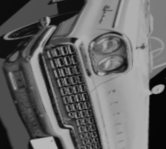
\includegraphics[width=0.30\textwidth]{images/Evaluation/Stereo_case/patch_1_ROI_of_template}
	}  \hspace{-2mm}
	\subfloat[Warped image for mercury plane]{
		\label{fig:Warped Image For Mercury Plane}
		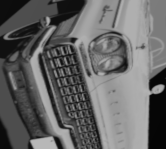
\includegraphics[width=0.30\textwidth]{images/Evaluation/Stereo_case/patch_1_ROI_of_warped_image}
	} \hspace{-2mm}
	\subfloat[Difference image]{
		\label{fig:Difference Image11}
		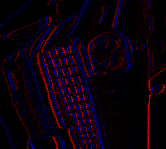
\includegraphics[width=0.30\textwidth]{images/Evaluation/Stereo_case/patch_1_difference}
	}\hspace{-2.5mm}
	\subfloat[]{
	%		\label{fig:diffBill}
	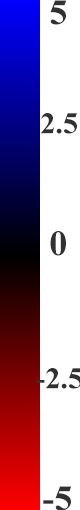
\includegraphics[height = 3.9cm]{./images/legendH}
} 
\\
	
		\subfloat[Template image]{
		\label{fig:Template Image21}
		
\includegraphics[width=0.30\textwidth]{images/Evaluation/Stereo_case/patch_2_ROI_of_template}
	}  \hspace{-2mm}
	\subfloat[Warped image for sheep plane]{
		\label{fig:Warped Image For Sheep Plane}
		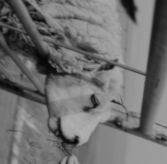
\includegraphics[width=0.30\textwidth]{images/Evaluation/Stereo_case/patch_2_ROI_of_warped_image}
	} \hspace{-2mm}
	\subfloat[Difference image]{
		\label{fig:Difference Image21}
		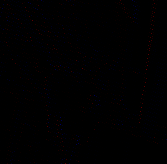
\includegraphics[width=0.30\textwidth]{images/Evaluation/Stereo_case/patch_2_difference}
	}\hspace{-2.5mm}
	\subfloat[]{
	%		\label{fig:diffBill}
	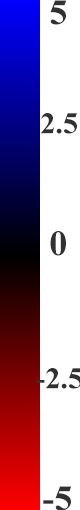
\includegraphics[height = 4.3cm]{./images/legendH}
} 
\\

		\subfloat[Template image]{
		\label{fig:Template Image211}
		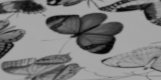
\includegraphics[width=0.30\textwidth]{images/Evaluation/Stereo_case/patch_3_ROI_of_template}
	}  \hspace{-2mm}
	\subfloat[Warped image for butterfly plane]{
		\label{fig:Warped Image For Butterfly Plane}
		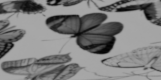
\includegraphics[width=0.30\textwidth]{images/Evaluation/Stereo_case/patch_3_ROI_of_warped_image}
	} \hspace{-2mm}
	\subfloat[Difference image]{
		\label{fig:Difference Image31}
		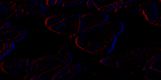
\includegraphics[width=0.30\textwidth]{images/Evaluation/Stereo_case/patch_3_difference}
	}\hspace{-2.5mm}
	\subfloat[]{
	%		\label{fig:diffBill}
	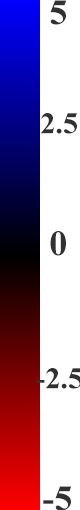
\includegraphics[height = 2.2cm]{./images/legendH}
} 

	\caption{Result of self-built stereo images}
	\label{fig:Result of Self-built Stereo Images}
\end{figure}

\begin{table}[tbp]
	\centering
	\scriptsize  
	\begin{tabular}{p{80pt} p{60pt}}
		\toprule
		Patch & {\bfseries PSNR(dB)}\\ \midrule
		Mercury Plane&  49.1514\\
		\addlinespace[3pt]
		Sheep Plane  &  66.9878\\
		\addlinespace[3pt]
		Butterfly Plane & 56.9686 \\ \bottomrule
	\end{tabular}
	\caption{PSNR of different patches for self-built stereo images}  
	\label{tab:PSNR of different patches for Self-built Stereo Images} 
\end{table}

\begin{table}[htbp]
	\centering
	\scriptsize  
	\begin{tabular}{p{80pt} p{60pt} p{60pt}}
		\toprule
		Patch & {\bfseries RMSD (pixel)} & {\bfseries Maximum(pixel)}\\ \midrule
		Mercury Plane&  0.044846&0.045849 \\
		\addlinespace[3pt]
		Sheep Plane  &  0.003704&0.004460 \\
		\addlinespace[3pt]
		Butterfly Plane & 0.017901&0.018868\\ \bottomrule
	\end{tabular}
	\caption{Displacement of different patches for self-built stereo images}  
	\label{tab:Displacement of different patches for self-built stereo images} 
\end{table}

\begin{table}[htbp]
	\centering
	\scriptsize  
	\begin{tabular}{ccc}
		\toprule
		\bfseries Parameter & \bfseries Ground Truth &\bfseries Estimated \\ \midrule
		$H_\infty$   &  $\begin{bmatrix}1 &0&0 \\
		0&1& 0\\
		0& 0&1\\ \end{bmatrix}$ &$\begin{bmatrix}1 &0&0 \\
		0&1& 0\\
		0& 0&1\\ \end{bmatrix}$  \\
		\addlinespace[5pt]
		$\rde$ & $\begin{bmatrix} -5.69822333e+02 \\
		-4.57549368e-03\\
		1.52790722e-05 \end{bmatrix}$&$\begin{bmatrix} -5.69822333e+02 \\
		-4.57549368e-03\\
		1.52790722e-05 \end{bmatrix}$ \\
		\addlinespace[5pt]
		$\vec{q}_1$ & $\begin{bmatrix} -5.04147145e-05 \\
		-2.53917154e-05\\
		1.22084579e-01 \end{bmatrix}$ & $\begin{bmatrix} -5.04285679e-05 \\
		-2.54000998e-05\\
		1.22014162e-01 \end{bmatrix} $ \\
		\addlinespace[5pt]
		$\vec{q}_2$ & $\begin{bmatrix} 6.80928394e-05\\
		-2.41470029e-05 \\
		4.64782197e-02 \end{bmatrix} $ & $\begin{bmatrix} 6.80857568e-05\\
		-2.41376373e-05 \\
		4.64747905e-02 \end{bmatrix}$ \\
		\addlinespace[5pt]
		$\vec{q}_3$ & $ \begin{bmatrix} 0.00000000e+00\\
		1.09855489e-04 \\
		3.28974882e-02 \end{bmatrix}$ & $\begin{bmatrix} -1.58691562e-09\\
		1.09810544e-04 \\
		3.28889686e-02 \end{bmatrix}$ \\
		${r_1}_1$ & &9.96429311e-01\\
		\addlinespace[5pt]
		${r_2}_1$& &  -2.65463250e-05\\
		\addlinespace[5pt]
		${r_1}_2$ & &9.94738600e-01\\
		\addlinespace[5pt]
		${r_2}_2$& & -4.20122298e-05\\
		\addlinespace[5pt]
		${r_1}_3$ & &9.97044402e-01\\
		\addlinespace[5pt]
		${r_2}_3$& & -2.07652871e-05\\
		\addlinespace[5pt]
		\bottomrule
	\end{tabular}
	\caption{Ground truth and estimated parameter for self-built stereo images}  
	\label{tab:Ground Truth and Estimated Parameter for self-built Stereo Images} 
\end{table}

\begin{figure}[tbp]
	\centering
	\subfloat[Template image]{
		\label{fig:temp1}
		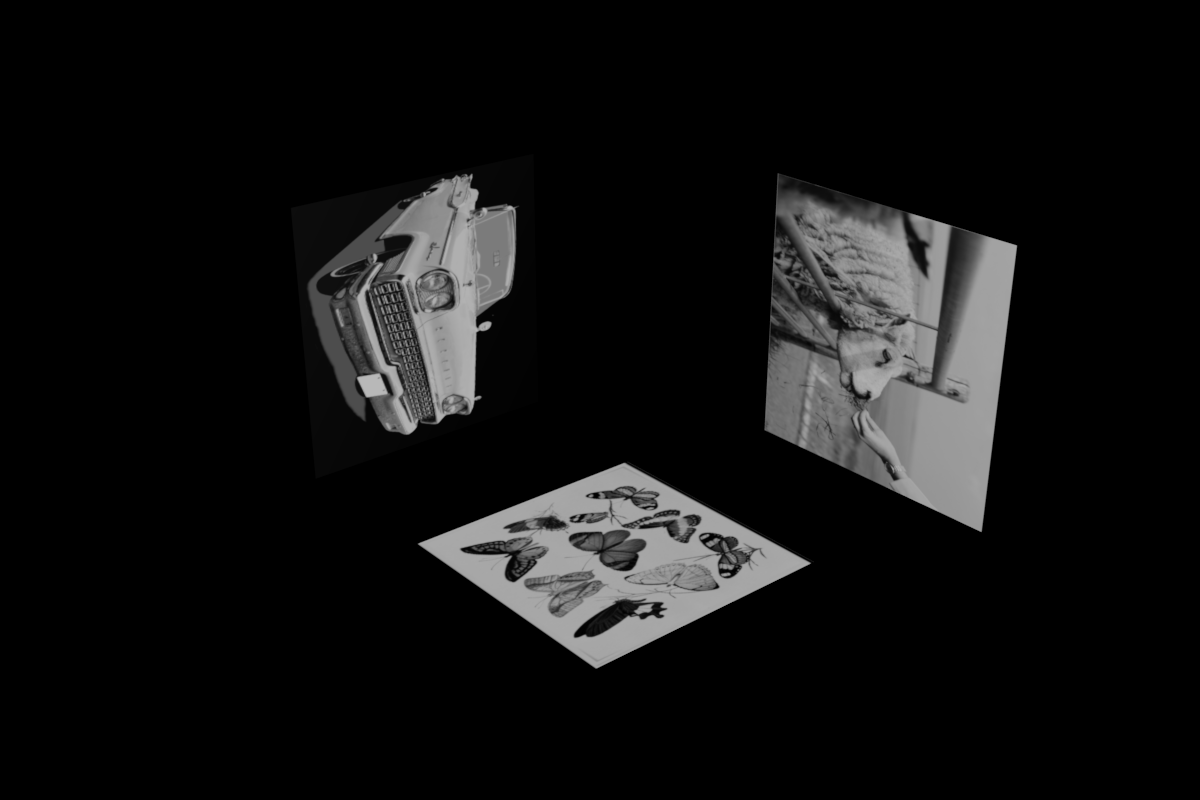
\includegraphics[width=0.40\textwidth]{./images/Evaluation/Stereo_case/original_template_img}
	} \quad
	\subfloat[Target image]{
		\label{fig:targ1}
		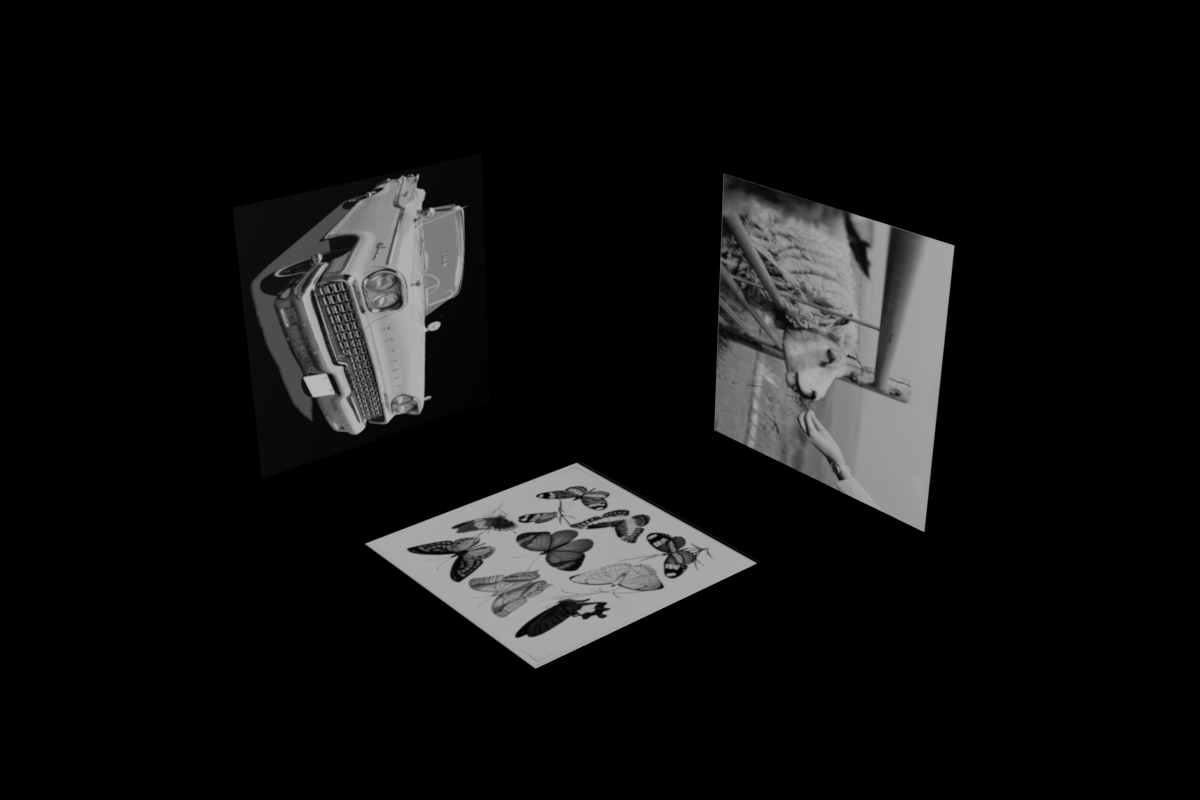
\includegraphics[width=0.40\textwidth]{./images/Evaluation/Stereo_case/original_target_img}
	} 
	\caption{Self-built stereo images}
	\label{fig:Self-built Stereo Images}
\end{figure}

\subsection{Testing with Self-built Normal Images}\label{subsec:Testing with Self-built Normal Images}
In this part, the results of testing with the self-built normal images are shown. I have chosen 3 image pairs to evaluate the algorithm.

First, a scenario with very different camera poses. The self-built images are shown in \cref{fig:Self-built Images(1)}. The ground truth and estimated parameters are in \cref{tab:Ground Truth and Estimated Parameter(1)}. PSNR is in \cref{tab:PSNR of different patches for Self-built Images(1)}. The root mean squared displacement (RMSD) and maximum displacement of all patches are shown in \cref{tab:Displacement of different patches for self-built images (1)}. The warped images are shown in \cref{fig:Result of Self-built Normal Images(1)}. From this result, we know that the result of brick-wall plane is not very good. The reason is that the algorithm sometimes responds to the texture structure not very well. In order to overcome it, we should use the image pyramid. 

What's more, the camera poses are very different and the algorithm can also find the correct result with suitable initialization. This proves that the algorithm can be applied on any two pictures, as long as they contain the same planes.
\begin{figure}[htbp]
	\centering
	\subfloat[Template image]{
		\label{fig:temp111}
		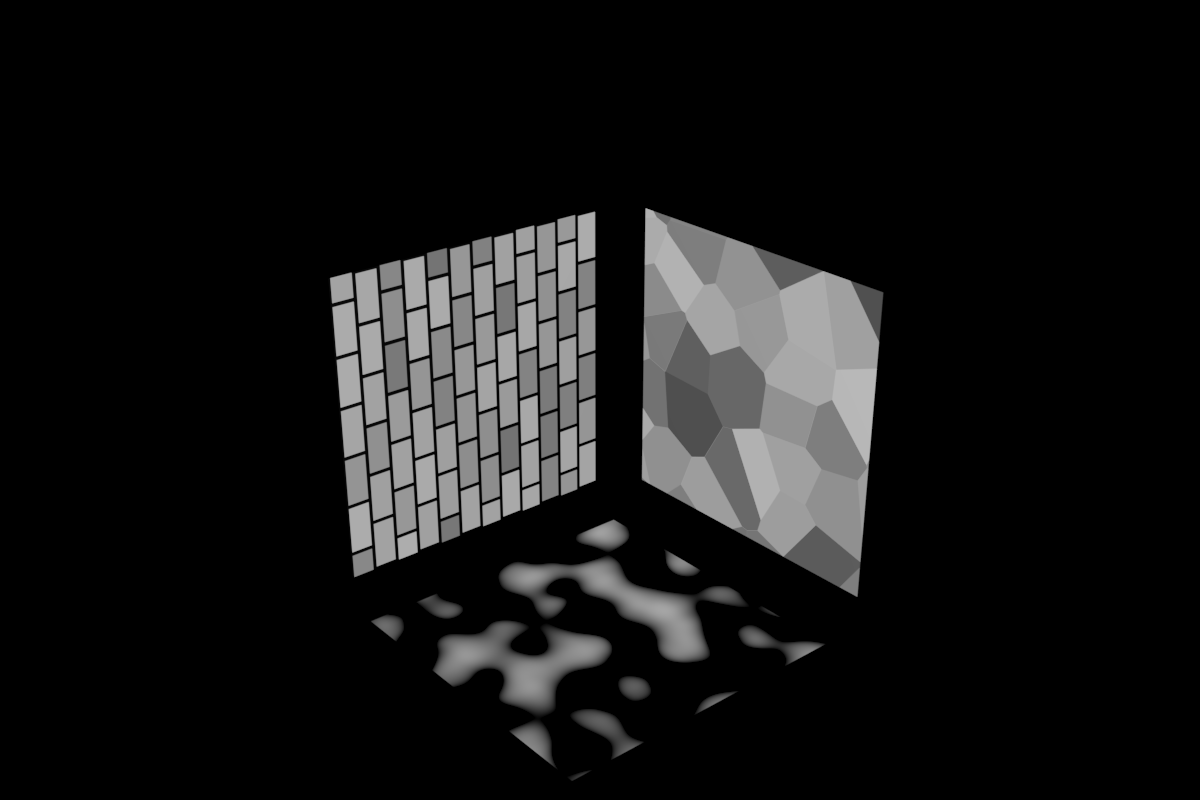
\includegraphics[width=0.40\textwidth]{./images/Evaluation/Normal_case1/original_template_img}
	} \quad
	\subfloat[Target image]{
		\label{fig:targ111}
		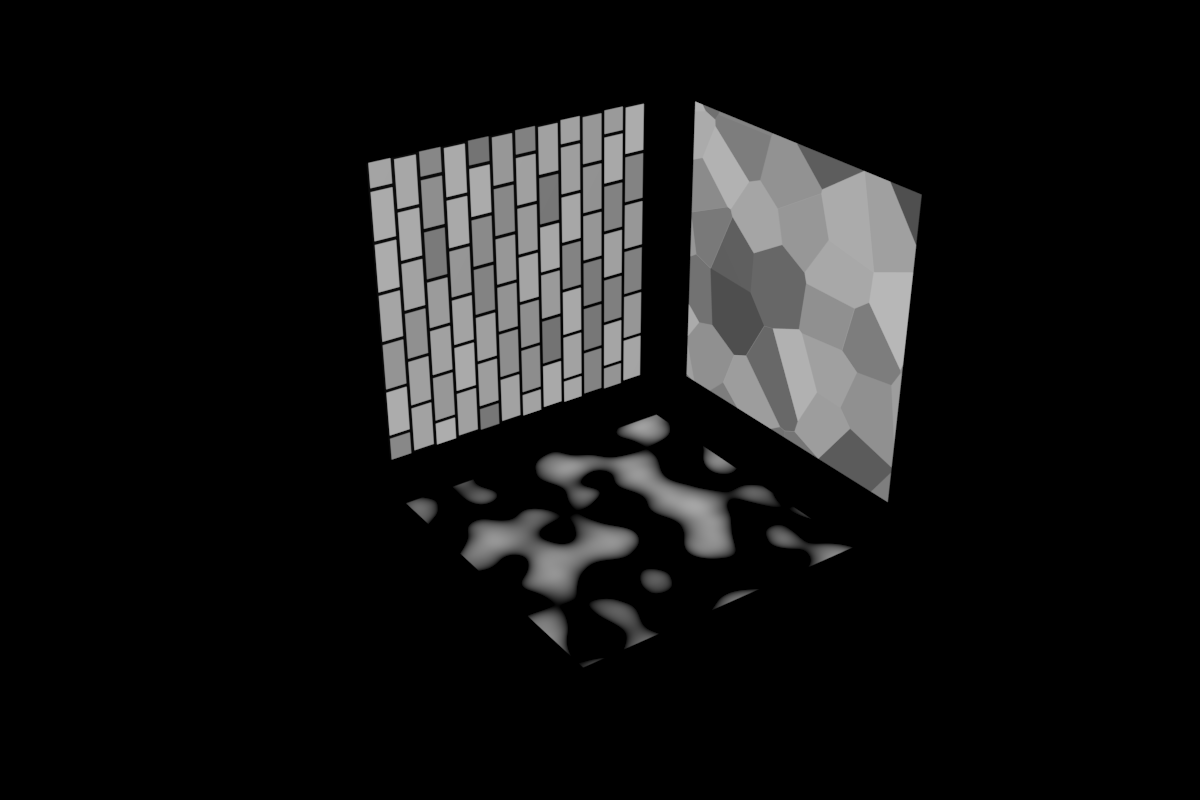
\includegraphics[width=0.40\textwidth]{./images/Evaluation/Normal_case1/original_target_img}
	} 
	\caption{Self-built images (1)}
	\label{fig:Self-built Images(1)}
\end{figure}

\begin{figure}[htbp]\centering
	\subfloat[Template image]{
		\label{fig:Template Image111}
		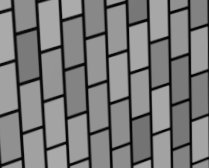
\includegraphics[width=0.30\textwidth]{images/Evaluation/Normal_case1/patch_1_ROI_of_template}
	} \hspace{-2mm} 
	\subfloat[Warped image for brick-wall plane]{
		\label{fig:Warped Image For Brick-wall Plane}
		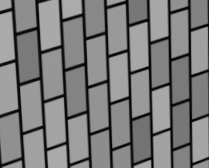
\includegraphics[width=0.30\textwidth]{images/Evaluation/Normal_case1/patch_1_ROI_of_warped_image}
	} \hspace{-2mm}
	\subfloat[Difference image]{
		\label{fig:Difference Image111}
		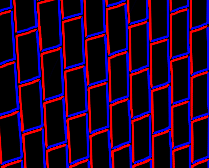
\includegraphics[width=0.30\textwidth]{images/Evaluation/Normal_case1/patch_1_difference}
	}\hspace{-2.5mm}
	\subfloat[]{
	%		\label{fig:diffBill}
	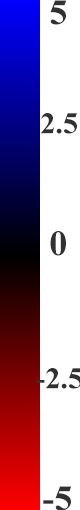
\includegraphics[height = 3.5cm]{./images/legendH}
} 
\\
	\subfloat[Template image]{
		\label{fig:Template Image2111}
		
\includegraphics[width=0.29\textwidth]{images/Evaluation/Normal_case1/patch_2_ROI_of_template}
	}  \hspace{-2mm}
	\subfloat[Warped image for voronoi plane]{
		\label{fig:Warped Image For Voronoi Plane}
		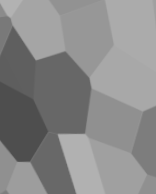
\includegraphics[width=0.29\textwidth]{images/Evaluation/Normal_case1/patch_2_ROI_of_warped_image}
	} \hspace{-2mm}
	\subfloat[Difference image]{
		\label{fig:Difference Image211}
		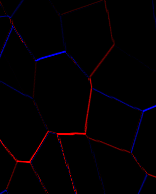
\includegraphics[width=0.29\textwidth]{images/Evaluation/Normal_case1/patch_2_difference}
	}\hspace{-2.5mm}
	\subfloat[]{
	%		\label{fig:diffBill}
	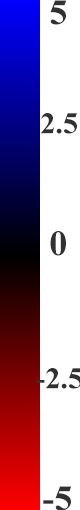
\includegraphics[height = 5.2cm]{./images/legendH}
} 
\\
	
	\subfloat[Template image]{
		\label{fig:Template Image21111}
		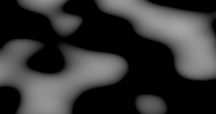
\includegraphics[width=0.30\textwidth]{images/Evaluation/Normal_case1/patch_3_ROI_of_template}
	}  \hspace{-2mm}
	\subfloat[Warped image for markov plane]{
	
		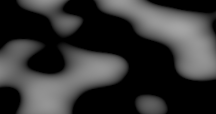
\includegraphics[width=0.30\textwidth]{images/Evaluation/Normal_case1/patch_3_ROI_of_warped_image}
	} \hspace{-2mm}
	\subfloat[Difference image]{
		\label{fig:Difference Image311}
		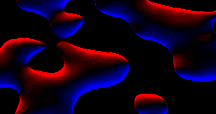
\includegraphics[width=0.30\textwidth]{images/Evaluation/Normal_case1/patch_3_difference}
	}\hspace{-2.5mm}
	\subfloat[]{
	%		\label{fig:diffBill}
	\includegraphics[height = 2.3cm]{./images/legendH}
} 
\\
	\caption{Result of self-built normal images (1)}
	\label{fig:Result of Self-built Normal Images(1)}
\end{figure}

\begin{table}[tbp]
	\centering
	\scriptsize  
	\begin{tabular}{p{80pt} p{60pt}}
		\toprule
		Patch & {\bfseries PSNR(dB)}\\ \midrule
		Brick-wall Plane&  29.3573\\
		\addlinespace[3pt]
		Voronoi Plane  &  40.4581\\
		\addlinespace[3pt]
		Markov Plane &38.8231 \\ \bottomrule
	\end{tabular}
	\caption{PSNR of different patches for self-built images (1)}  
	\label{tab:PSNR of different patches for Self-built Images(1)} 
\end{table}

\begin{table}[htbp]
	\centering
	\scriptsize 
	\begin{tabular}{p{80pt} p{60pt} p{60pt}}
		\toprule
		Patch & {\bfseries RMSD (pixel)} & {\bfseries Maximum(pixel)}\\ \midrule
		Brick-wall Plane&  0.304703&0.325780 \\
		\addlinespace[3pt]
		Voronoi Plane  &  0.208013&0.277421 \\
		\addlinespace[3pt]
		Markov Plane & 0.344370&0.397986 \\ 
		\addlinespace[3pt]
		All Patches & 0.288475&0.397986 \\ \bottomrule
	\end{tabular}
	\caption{Displacement of different patches for self-built images (1)}  
	\label{tab:Displacement of different patches for self-built images (1)} 
\end{table}

\begin{table}[htbp]
	\centering
	\tiny 
	\begin{tabular}{ccc}
		\toprule
		\bfseries Parameter & \bfseries Ground Truth &\bfseries Estimated \\ \midrule
		$H_\infty$   &  $\begin{bmatrix}9.65703446e-01 &-8.36839711e-03&1.39138794e+02 \\
		2.19264412e-02&1.01576119e+00& -1.23767980e+02\\
		-5.08187535e-05& 4.74420190e-05&1.00606213e+00 \end{bmatrix}$ &$\begin{bmatrix}9.65839836e-01 &-8.41589335e-03 & 1.39060980e+02 \\
		2.19485280e-02 & 1.01520898e+00& -1.23718912e+02\\
		-5.05974374e-05  &4.74229252e-05 & 1.00579468e+00 \end{bmatrix}$  \\
		\addlinespace[5pt]
		$\rde$ & $\begin{bmatrix} -7.24246259e+02 \\
		-1.64515557e+01\\
		3.81296513e-02 \end{bmatrix}$&$\begin{bmatrix} -7.24204197e+02 \\
		-1.64534715e+01\\
		4.01498913e-02 \end{bmatrix}$ \\
		\addlinespace[5pt]
		$\vec{q}_1$ & $\begin{bmatrix} -5.96261061e-05 \\
		-3.00310957e-05\\
		1.44390941e-01 \end{bmatrix}$ & $\begin{bmatrix} -5.96507588e-05 \\
		-3.02164145e-05\\
		1.44743346e-01 \end{bmatrix}$ \\
		\addlinespace[5pt]
		$\vec{q}_2$ & $\begin{bmatrix}8.15476596e-05 \\-2.89183354e-05 \\ 5.56620941e-02\end{bmatrix}$ & $\begin{bmatrix}  8.14932969e-05\\
		-2.88990747e-05\\
		5.57176245e-02 \end{bmatrix}$ \\
		\addlinespace[5pt]
		$\vec{q}_3$ & $\begin{bmatrix} 0.00000000e+00  \\1.15523713e-04 \\ 3.45949029e-02 \end{bmatrix}$ & $\begin{bmatrix}1.89395051e-07\\
		1.14948256e-04\\
		3.49029342e-02 \end{bmatrix}$ \\
		${r_1}_1$ & &9.93390769e-01\\
		\addlinespace[5pt]
		${r_2}_1$& & -4.61817515e-05\\
		\addlinespace[5pt]
		${r_1}_2$ & &9.97370299e-01\\
		\addlinespace[5pt]
		${r_2}_2$& & -1.80821342e-05\\
		\addlinespace[5pt]
		${r_1}_2$ & &9.96350068e-01\\
		\addlinespace[5pt]
		${r_2}_2$& & -3.17773268e-05\\
		\addlinespace[5pt]
		\bottomrule
	\end{tabular}
	\caption{Ground truth and estimated parameter (1)}  
	\label{tab:Ground Truth and Estimated Parameter(1)} 
\end{table}

The second example images pair comes from two cameras with very different poses, too. The self-built images are shown in \cref{fig:Self-built Images(2)}. The ground truth and estimated parameters are in \cref{tab:Ground Truth and Estimated Parameter(2)}. PSNR is in \cref{tab:PSNR of different patches for Self-built Images(2)}.  The root mean squared displacement (RMSD) and maximum displacement of all patches are shown in \cref{tab:Displacement of different patches for self-built images (2)}. The warped images are shown in \cref{fig:Result of Self-built Normal Images(2)}.  There are no texture structure in these images. So the result is all perfect.

\begin{figure}[htbp]
	\centering
	\subfloat[Template image]{
		\label{fig:temp1sdf11}
		\includegraphics[width=0.40\textwidth]{./images/Evaluation/Normal_case3/original_template_img}
	} \quad
	\subfloat[Target image]{
		\label{fig:targ11dwe1}
		\includegraphics[width=0.40\textwidth]{./images/Evaluation/Normal_case3/original_target_img}
	} 
	\caption{Self-built images (2)}
	\label{fig:Self-built Images(2)}
\end{figure}

\begin{figure}[htbp]\centering
	\subfloat[Template image]{
		\label{fig:Template Image1daf11}
		\includegraphics[width=0.30\textwidth]{images/Evaluation/Normal_case3/patch_1_ROI_of_template}
	}\hspace{-2mm}
	\subfloat[Warped image for fantasy plane]{
	
		\includegraphics[width=0.30\textwidth]{images/Evaluation/Normal_case3/patch_1_ROI_of_warped_image}
	}\hspace{-2mm}
	\subfloat[Difference image]{
		\label{fig:Difference Image1we11}
		\includegraphics[width=0.30\textwidth]{images/Evaluation/Normal_case3/patch_1_difference}
	}\hspace{-2.5mm}
	\subfloat[]{
	%		\label{fig:diffBill}
	\includegraphics[height = 3.2cm]{./images/legendH}
} \\
	
	\subfloat[Template image]{
		\label{fig:Template Image2we111}
		\includegraphics[width=0.30\textwidth]{images/Evaluation/Normal_case3/patch_2_ROI_of_template}
	}\hspace{-2mm}
	\subfloat[Warped image for squirrel plane]{
		\label{fig:Warped Image For Vordsfaonoi Plane}
		\includegraphics[width=0.30\textwidth]{images/Evaluation/Normal_case3/patch_2_ROI_of_warped_image}
	}\hspace{-2mm}
	\subfloat[Difference image]{
		\label{fig:Difference Image2we11}
		\includegraphics[width=0.30\textwidth]{images/Evaluation/Normal_case3/patch_2_difference}
	}\hspace{-2.5mm}
	\subfloat[]{
	%		\label{fig:diffBill}
	\includegraphics[height = 4.7cm]{./images/legendH}
} \\
	\subfloat[Template image]{
		\label{fig:Template Image21we111}
		\includegraphics[width=0.30\textwidth]{images/Evaluation/Normal_case3/patch_3_ROI_of_template}
	}\hspace{-2mm}  
	\subfloat[Warped image for sparrow plane]{
		\label{fig:Warped Image For Marwekov Planweqwee}
		\includegraphics[width=0.30\textwidth]{images/Evaluation/Normal_case3/patch_3_ROI_of_warped_image}
	}\hspace{-2mm}
	\subfloat[Difference image]{
		\label{fig:Difference Image3we11}
		\includegraphics[width=0.30\textwidth]{images/Evaluation/Normal_case3/patch_3_difference}
	}\hspace{-2.5mm}
	\subfloat[]{
	%		\label{fig:diffBill}
	\includegraphics[height = 3.4cm]{./images/legendH}
} 

	\caption{Result of self-built normal images (2)}
	\label{fig:Result of Self-built Normal Images(2)}
\end{figure}

\begin{table}[tbp]
	\centering
	\scriptsize  
	\begin{tabular}{p{80pt} p{60pt}}
		\toprule
		Patch & {\bfseries PSNR(dB)}\\ \midrule
		Fantasy Plane&  36.1911\\
		\addlinespace[3pt]
		Squirrel Plane  &  40.2400\\
		\addlinespace[3pt]
		Sparrow Plane &40.4210\\ \bottomrule
	\end{tabular}
	\caption{PSNR of different patches for self-built images (2)}  
	\label{tab:PSNR of different patches for Self-built Images(2)} 
\end{table}

\begin{table}[htbp]
	\centering
	\scriptsize 
	\begin{tabular}{p{80pt} p{60pt} p{60pt}}
		\toprule
		Patch & {\bfseries RMSD (pixel)} & {\bfseries Maximum(pixel)}\\ \midrule
		Fantasy Plane&  0.291320&0.393618 \\
		\addlinespace[3pt]
		Squirrel Plane  &  0.131122&0.154218 \\
		\addlinespace[3pt]
		Sparrow Plane & 0.189493&0.207162 \\ 
		\addlinespace[3pt]
		All Patches & 0.202340&0.393618 \\ \bottomrule
	\end{tabular}
	\caption{Displacement of different patches for self-built images (2)}  
	\label{tab:Displacement of different patches for self-built images (2)} 
\end{table}

\begin{table}[htbp]
	\centering
	\tiny 
	\begin{tabular}{ccc}
		\toprule
		\bfseries Parameter & \bfseries Ground Truth &\bfseries Estimated \\ \midrule
		$H_\infty$   &  $\begin{bmatrix}9.52824171e-01& -1.61137624e-01&  2.06105992e+02 \\
		1.88784031e-01&  1.00060579e+00 &-2.35871911e+02\\
		-4.01833405e-05 & 6.27021960e-05 & 9.92769988e-01 \end{bmatrix}$ &$\begin{bmatrix}9.51958568e-01& -1.61028691e-01&  2.05291642e+02 \\
		1.88447546e-01&  9.99411077e-01 &-2.35358036e+02\\
		-3.99424923e-05&  6.26078118e-05&  9.90950379e-01 \end{bmatrix}$  \\
		\addlinespace[5pt]
		$\rde$ & $\begin{bmatrix} -1.21556156e+03 \\-4.60188500e+01\\ -7.75948410e-02 \end{bmatrix}$&$\begin{bmatrix} -1.21004890e+03\\
		-4.60502141e+01\\
		-7.27863792e-02 \end{bmatrix}$ \\
		\addlinespace[5pt]
		$\vec{q}_1$ & $\begin{bmatrix} -3.18191743e-05\\ -3.30706122e-06\\  1.00547129e-01 \end{bmatrix}$ & $\begin{bmatrix} -3.20962545e-05\\
		-4.33730691e-06\\
		1.00806139e-01 \end{bmatrix}$ \\
		\addlinespace[5pt]
		$\vec{q}_2$ & $\begin{bmatrix}5.10113553e-05\\ -1.23551078e-05 \\ 5.98174870e-02\end{bmatrix}$ & $\begin{bmatrix}   5.10028797e-05\\
		-1.23051622e-05\\
		5.98152421e-02 \end{bmatrix}$ \\
		\addlinespace[5pt]
		$\vec{q}_3$ & $\begin{bmatrix} 1.06495815e-05  \\4.19802260e-05 \\ 7.33070552e-02 \end{bmatrix}$ & $\begin{bmatrix}1.05603440e-05\\
		4.18628465e-05\\
		7.33696013e-02 \end{bmatrix}$ \\
		${r_1}_1$ & &1.01451717e+00\\
		\addlinespace[5pt]
		${r_2}_1$& & 1.17515309e-04\\
		\addlinespace[5pt]
		${r_1}_2$ & & 9.86832299e-01\\
		\addlinespace[5pt]
		${r_2}_2$& & -1.10771571e-04\\
		\addlinespace[5pt]
		${r_1}_2$ & &9.96963583e-01\\
		\addlinespace[5pt]
		${r_2}_2$& & -1.98783474e-05\\
		\addlinespace[5pt]
		\bottomrule
	\end{tabular}
	\caption{Ground truth and estimated parameter (2)}  
	\label{tab:Ground Truth and Estimated Parameter(2)} 
\end{table}

Finally, I show a result of a pair of unrectified stereo images. The self-built images are shown in \cref{fig:Self-built Images(3)}. The ground truth and estimated parameters are in \cref{tab:Ground Truth and Estimated Parameter(3)}. PSNR is in \cref{tab:PSNR of different patches for Self-built Images(3)}. The root mean squared displacement (RMSD) and maximum displacement of all patches are shown in \cref{tab:Displacement of different patches for self-built images (3)}. The warped images are shown in \cref{fig:Result of Self-built Normal Images(3)}.

\begin{figure}[htbp]
	\centering
	\subfloat[Template image]{
		\label{fig:temp1sdf1we1}
		\includegraphics[width=0.40\textwidth]{./images/Evaluation/Normal_case4/original_template_img}
	} \quad
	\subfloat[Target image]{
		\label{fig:targ11dewe1}
		\includegraphics[width=0.40\textwidth]{./images/Evaluation/Normal_case4/original_target_img}
	} 
	\caption{Self-built images (3)}
	\label{fig:Self-built Images(3)}
\end{figure}

\begin{figure}[htbp]\centering
	\subfloat[Template image]{
		\label{fig:Template Imsdage1daf11}
		\includegraphics[width=0.30\textwidth]{images/Evaluation/Normal_case4/patch_1_ROI_of_template}
	}\hspace{-2mm}
	\subfloat[Warped image for fox plane]{
		\label{fig:Warped Image For Bricwewek-wall Plane}
		\includegraphics[width=0.30\textwidth]{images/Evaluation/Normal_case4/patch_1_ROI_of_warped_image}
	}\hspace{-2mm}
	\subfloat[Difference image]{
		\label{fig:Difference Imawege1we11}
		\includegraphics[width=0.30\textwidth]{images/Evaluation/Normal_case4/patch_1_difference}
	}\hspace{-2.5mm}
	\subfloat[]{
	%		\label{fig:diffBill}
	\includegraphics[height = 3.6cm]{./images/legendH}
} \\
	
	\subfloat[Template image]{
		\label{fig:Template Imagewe2we111}
		\includegraphics[width=0.30\textwidth]{images/Evaluation/Normal_case4/patch_2_ROI_of_template}
	}\hspace{-2mm}
	\subfloat[Warped image for eiffel plane]{
		\label{fig:Warped Image For Vordswefaonoi Plane}
		\includegraphics[width=0.30\textwidth]{images/Evaluation/Normal_case4/patch_2_ROI_of_warped_image}
	}\hspace{-2mm}
	\subfloat[Difference image]{
		\label{fig:Difference Imawege2we11}
		\includegraphics[width=0.30\textwidth]{images/Evaluation/Normal_case4/patch_2_difference}
	}\hspace{-2.5mm}
	\subfloat[]{
	%		\label{fig:diffBill}
	\includegraphics[height = 4.2cm]{./images/legendH}
} \\
	
	\subfloat[Template image]{
		\label{fig:Template Imawege21we111}
		\includegraphics[width=0.30\textwidth]{images/Evaluation/Normal_case4/patch_3_ROI_of_template}
	}\hspace{-2mm}
	\subfloat[Warped image for greece plane]{
		\label{fig:Warped Image For Marwewerqwer23232kov Plane}
		\includegraphics[width=0.30\textwidth]{images/Evaluation/Normal_case4/patch_3_ROI_of_warped_image}
	}\hspace{-2mm}
	\subfloat[Difference image]{
		\label{fig:Difference Imweage3we11}
		\includegraphics[width=0.30\textwidth]{images/Evaluation/Normal_case4/patch_3_difference}
	}\hspace{-2.5mm}
	\subfloat[]{
	%		\label{fig:diffBill}
	\includegraphics[height = 3.3cm]{./images/legendH}
} 
	\caption{Result of self-built normal images (3)}
	\label{fig:Result of Self-built Normal Images(3)}
\end{figure}

\begin{table}[tbp]
	\centering
	\scriptsize  
	\begin{tabular}{p{80pt} p{60pt}}
		\toprule
		Patch & {\bfseries PSNR(dB)}\\ \midrule
		Fox Plane&  46.1314\\
		\addlinespace[3pt]
		Eiffel Plane  &  44.7784\\
		\addlinespace[3pt]
		Greece Plane &32.3565\\ \bottomrule
	\end{tabular}
	\caption{PSNR of different patches for self-built images (3)}  
	\label{tab:PSNR of different patches for Self-built Images(3)} 
\end{table}

\begin{table}[htbp]
	\centering
	\scriptsize  
	\begin{tabular}{p{80pt} p{60pt} p{60pt}}
	\toprule
	Patch & {\bfseries RMSD (pixel)} & {\bfseries Maximum(pixel)}\\ \midrule
	Fox Plane&  0.126497&0.226566 \\
	\addlinespace[3pt]
	Eiffel Plane  &  0.087420&0.162986\\
	\addlinespace[3pt]
	Greece Plane & 0.136024&0.194004 \\ 
	\addlinespace[3pt]
	All Patches & 0.117115&0.226566 \\ \bottomrule
	\end{tabular}
	\caption{Displacement of different patches for self-built images (3)}  
	\label{tab:Displacement of different patches for self-built images (3)} 
\end{table}

\begin{table}[htbp]
	\centering
	\tiny
	\begin{tabular}{ccc}
		\toprule
		\bfseries Parameter & \bfseries Ground Truth &\bfseries Estimated \\ \midrule
		$H_\infty$   &  $\begin{bmatrix}9.67030208e-01& -3.13227134e-02 & 1.42036819e+02 \\
		1.54081860e-02 & 1.00157007e+00 &-1.94949553e+01\\
		-4.93452978e-05&  5.50999444e-06 & 1.02462584e+00 \end{bmatrix}$ &$\begin{bmatrix}9.89508997e-01& -3.14215411e-02  &1.41579233e+02 \\
		1.61180210e-02&  1.02097858e+00& -2.02384459e+01\\
		-4.89309883e-05&  6.50245995e-06&  1.03992663e+00 \end{bmatrix}$  \\
		\addlinespace[5pt]
		$\rde$ & $\begin{bmatrix} -1.19028099e+03 \\-1.55712365e+00\\  4.98674731e-03 \end{bmatrix}$&$\begin{bmatrix} -1.19003604e+03\\
		-1.62088391e+00\\
		3.23745088e-02 \end{bmatrix}$ \\
		\addlinespace[5pt]
		$\vec{q}_1$ & $\begin{bmatrix}-4.45934748e-05\\ -2.22353073e-05\\  1.08137896e-01 \end{bmatrix}$ & $\begin{bmatrix} -4.18794095e-05\\
		2.10081204e-05\\
		1.07554103e-01 \end{bmatrix}$ \\
		\addlinespace[5pt]
		$\vec{q}_2$ & $\begin{bmatrix}4.89262638e-05\\ -1.18500922e-05 \\ 5.73724445e-02\end{bmatrix}$ & $\begin{bmatrix}   5.09498850e-05\\
		-1.22376789e-05\\
		5.80580159e-02 \end{bmatrix}$ \\
		\addlinespace[5pt]
		$\vec{q}_3$ & $\begin{bmatrix}-1.00128972e-05\\  1.09754268e-05\\  9.83050209e-02 \end{bmatrix}$ & $\begin{bmatrix}-7.76330602e-06\\
		1.09390874e-05\\
		9.86232716e-02 \end{bmatrix}$ \\
		${r_1}_1$ & &9.99853298e-01\\
		\addlinespace[5pt]
		${r_2}_1$& & -1.25598370e-06\\
		\addlinespace[5pt]
		${r_1}_2$ & & 9.94348907e-01\\
		\addlinespace[5pt]
		${r_2}_2$& & -3.45616975e-05\\
		\addlinespace[5pt]
		${r_1}_2$ & &1.02688585e+00\\
		\addlinespace[5pt]
		${r_2}_2$& & 1.64952502e-04\\
		\addlinespace[5pt]
		\bottomrule
	\end{tabular}
	\caption{Ground truth and estimated parameter (3)}  
	\label{tab:Ground Truth and Estimated Parameter(3)} 
\end{table}

\clearpage

\subsection{Comparison and analysis}
So far, the proposed algorithm is applied to the self-built images and Middlebury Stereo Vision Datasets. The specific test results obtained are listed in detail in \cref{subsec:Testing with Middlebury Stereo Vision Datasets}, \cref{subsec:Testing with Self-built Stereo Images},  \cref{subsec:Testing with Self-built Normal Images}, \cref{subsec:Rectified Stereo Images} and \cref{subsec:Unrectified Images}. For datasets with ground truth, we can analyze our algorithm by comparing the estimated result with the ground truth.

I summarize all the results of image pairs with ground truth in \cref{tab:Result of rectified stereo testing images} and \cref{tab:Result of unrectified testing images}.

\begin{table}[htbp]
	\centering
	\scriptsize   
	\begin{tabular}{ccccc}
		\toprule
		Image Pair & Patch & {\bfseries RMSD (pixel)} & {\bfseries Maximum(pixel)}&{\bfseries PSNR(dB)}\\ \midrule
		\multirow{6}{80pt}{\centering \cref{fig:Template and transformed plane patches in Middlebury Stereo Vision Datasets (1)}}&(1)&  2.252596&3.125&37.5768\\
		\addlinespace[3pt]
		&(2)  &  0.647761&0.975361&40.4451 \\
		\addlinespace[3pt]
		&(3) & 0.184386&0.324421&45.9940\\ 
		\addlinespace[3pt]
		&(4)& 0.536102&0.859401& 42.4099 \\ 
		\addlinespace[3pt]
		&(5)& 0.954197& 2.257174& 47.7764 \\ 
		\addlinespace[3pt]
		&(6)& 0.895281&1.001767& 38.3245 \\
		\addlinespace[6pt]
		
		\multirow{6}{80pt}{\centering \cref{fig:Template and transformed plane patches in Middlebury Stereo Vision Datasets (2)}}&(1)& 0.203423&0.441505&46.9869 \\
		\addlinespace[3pt]
		&(2)  & 1.123935&2.192497&41.8912 \\
		\addlinespace[3pt]
		&(3) &1.523684&2.625&32.6315 \\ 
		\addlinespace[3pt]
		&(4)&0.358562&0.483073& 41.8892 \\ 
		\addlinespace[3pt]
		&(5)& 1.111534&1.700925& 36.9338\\ 
		\addlinespace[3pt]
		&(6)&0.102031&0.290172&49.0576 \\
		\addlinespace[6pt]
		
		\multirow{5}{80pt}{\centering \cref{fig:Template and transformed plane patches in Middlebury Stereo Vision Datasets (3)}}&(1)&0.507921&0.883605& 51.4393 \\
		\addlinespace[3pt]
		&(2)  & 0.344584&0.689927&44.9664 \\
		\addlinespace[3pt]
		&(3) &1.353465&3.046611&34.9695 \\ 
		\addlinespace[3pt]
		&(4)&0.664646&1.188368& 47.4049 \\ 
		\addlinespace[3pt]
		&(5)& 0.188721&0.554017& 45.2209\\ 		
		\addlinespace[6pt]
		
		\multirow{3}{80pt}{\centering \cref{fig:Result of Self-built Stereo Images}}&Mercury Plane& 0.044846&0.045849&49.1514 \\
		\addlinespace[3pt]
		&Sheep Plane  &  0.003704&0.004460&66.9878\\
		\addlinespace[3pt]
		&Butterfly Plane &  0.017901&0.018868&56.9686 \\ 		
		\bottomrule
	\end{tabular}
	\caption{Result of rectified stereo testing images}  
	\label{tab:Result of rectified stereo testing images} 
\end{table}

From \cref{tab:Result of rectified stereo testing images}, we can see that the results of applying the proposed algorithm to self-built stereo images are significantly better than the Middlebury Stereo Vision datasets. The difference is that we have the 100 $\%$ right ground truth of self-build stereo images,  but we only have a disparity map scaled by a factor of 8, which means that a value of 80 in disparity map presents that the corresponding pixel in template image is 10 pixels to the right of target image. In this case, the pixel value in disparity map is only integer, the final ground truth got is not 100 $\%$ accurate. Even so, our average error is only less than half or at most one pixels. What's more, the rectangular areas we manually selected in Middlebury Stereo Vision Datasets may not all be the same plane, which will also cause inaccurate results.

 \begin{table}[htbp]
 	\centering
 	\scriptsize   
 	\begin{tabular}{ccccc}
 		\toprule
 		Image Pair & Patch & {\bfseries RMSD (pixel)} & {\bfseries Maximum(pixel)}&{\bfseries PSNR(dB)}\\ \midrule
 		\multirow{4}{80pt}{\centering \cref{fig:Result of Unrectified Images}}&Deer Plane&  0.186577&0.370456&44.9857 \\
 		\addlinespace[3pt]
 		&Flower Plane  &  0.130046&0.162404&38.3061 \\
 		\addlinespace[3pt]
 		&Cat Plane & 0.369888&0.874363&41.5518 \\ 
 		\addlinespace[3pt]
 		&All Patches & 0.215594&0.874363& - \\ 
 		\addlinespace[6pt]
 		
 		\multirow{4}{80pt}{\centering \cref{fig:Result of Self-built Normal Images(1)}}&Brick-wall Plane&  0.304703&0.325780&29.3573 \\
 		\addlinespace[3pt]
 		&Voronoi Plane  &  0.208013&0.277421&40.4581 \\
 		\addlinespace[3pt]
 		&Markov Plane & 0.344370&0.397986&38.8231 \\ 
 		\addlinespace[3pt]
 		&All Patches & 0.288475&0.397986&- \\
 		\addlinespace[6pt]
 		
 		\multirow{4}{80pt}{\centering \cref{fig:Result of Self-built Normal Images(2)}}&Fantasy Plane&  0.291320&0.393618&36.1911 \\
 		\addlinespace[3pt]
 		&Squirrel Plane  &  0.131122&0.154218&40.2400 \\
 		\addlinespace[3pt]
 		&Sparrow Plane & 0.189493&0.207162&40.4210 \\ 
 		\addlinespace[3pt]
 		&All Patches & 0.202340&0.393618&- \\
 		\addlinespace[6pt]
 		
 		\multirow{4}{80pt}{\centering \cref{fig:Result of Self-built Normal Images(3)}}&Fox Plane&  0.126497&0.226566&46.1314 \\
 		\addlinespace[3pt]
 		&Eiffel Plane  &  0.087420&0.162986&44.7784\\
 		\addlinespace[3pt]
 		&Greece Plane & 0.136024&0.194004&32.3565 \\ 
 		\addlinespace[3pt]
 		&All Patches & 0.117115&0.226566&- \\
 		\bottomrule
 	\end{tabular}
 	\caption{Result of unrectified testing images}  
 	\label{tab:Result of unrectified testing images} 
 \end{table}

I show this four unrectified self-built image pairs because they all have their own characteristics and can be used to represent most of the application scenarios. The angle between the cameras of \cref{fig:Result of Unrectified Images} is very small. Comparing to this, the angle between the cameras of \cref{fig:Result of Self-built Normal Images(3)} is a little bit bigger. The Results of these are both acceptable. This proves that the pose of the cameras has little or no influence of the proposed algorithm.

The angles between cameras of \cref{fig:Result of Unrectified Images} and \cref{fig:Result of Self-built Normal Images(1)} are both small. But the plane objects in the images are not the same type. \cref{fig:Result of Unrectified Images} has synthetic textures whereas the other has real images. And there is also a repeating structure in brick-wall plane in \cref{fig:Result of Unrectified Images}. It's obviously that the result of repeating structure is not good as another. And the contains of the plane objects has small influence.

\cref{fig:Result of Self-built Normal Images(1)} has standard orthogonal planes whereas the other three have arbitrary angle between them. More precisely,  \cref{fig:Result of Unrectified Images} has near orthogonal planes. \cref{fig:Result of Self-built Normal Images(2)} and \cref{fig:Result of Self-built Normal Images(3)} have near parallel planes in contrast. But the results of the proposed algorithm are almost the same. We can conclude that the pose or position of target plane doesn't influence the result of the proposed algorithm.

